\documentclass[12pt,a4paper,twoside]{article}
\usepackage{times}	% Skalierbarer und lesbarer Zeichensatz
\usepackage{ucs}	% Benötigt für Eingabe von unicode-Zeichensätzen
\usepackage[utf8x]{inputenc} % Aktiviert Eingabe von unicode-Zeichensätzen
\usepackage{epsfig}	% Makros zum Einfügen von Grafiken
\usepackage{anysize}	% Makros zum Einstellen der Seitenränder
%\usepackage{makeidx}	% Makros zum Erstellen des Indexes
\usepackage{url}
\usepackage{hyperref}
\usepackage{fancyhdr}
\usepackage{listings}
\usepackage{color}
\usepackage{comment}

\marginsize{30mm}{20mm}{20mm}{20mm}  % Seitenränder links, rechts, oben, unten
\parindent0em		% Keine amerikanische Einrückung am Anfang von Paragraphen
\renewcommand{\floatpagefraction}{.99}

\pagestyle{fancy}	% Seitenstil
%\makeindex		% wird für Erstellung von Stichwortverzeichnissen benötigt

% Ende der Voreinstellungen

\newcommand{\paperversion}{{\em Version 1.01}}

\fancyhead{}
\fancyhead[LE,RO]{page \thepage\ of \pageref{LastPage}}
\fancyhead[LO,RE]{\nouppercase{\rightmark}}
\renewcommand{\sectionmark}[1]{\markboth{#1}{#1}}
\renewcommand{\subsectionmark}[1]{}

\renewcommand{\footrulewidth}{0.4pt}
\fancyfoot{}
\fancyfoot[LE,RO]{dvdisaster codec specification}
\fancyfoot[LO]{created: \today}
\fancyfoot[RE]{\paperversion}

\newcommand{\projectversion}{0.79.6}


\begin{document}

\definecolor{lightblue}{RGB}{224,224,255}
\pagecolor{lightblue}
\title{The dvdisaster Reed-Solomon Codec specification}
\author{The dvdisaster development team\\support@dvdisaster.org}
\date{}
\maketitle
\thispagestyle{empty}

\centerline{
\includegraphics[width=32mm]{title.eps}}
  
\begin{center}
\paperversion
\end{center}

\bigskip

\begin{abstract}
This is the {\em blue manual}, describing the data formats of the dvdisaster
Reed-Solomon codecs which are currently called RS01, RS02 and RS03.
The codecs create Reed-Solomon parity data to protect data stored on optical media.
Depending on the codec, parity data can either be stored in a separate file 
or be integrated with the .iso image on the same medium. 
See \homepage for additional resources on the dvdisaster pro\-ject,
e.g. for the {\em orange manual} (manual.pdf) containing information for end users.
\end{abstract}

\bigskip

{\bf Target audience.} This paper is primarily intended as a working base for the
dvdisaster developers and, when the final version has been crafted, as an implementation
guide for third party developers who wish to create and process dvdisaster error correction data.
It is {\bf neither intended nor suitable} as end-user documentation; for usage information
please refer to the online documentation at \homepage.

\bigskip

{\bf Prerequisites.} This paper assumes profound knowledge of coding theory and the 
underlying math. The reader is assumed to have a thorough understanding of Reed-Solomon
codes, both in theory and from an implementation viewpoint. A basic understanding
of programming in C is also assumed.

\vfill
\begin{center}
{\em 
Copyright 2008-2015 Carsten Gnörlich.\\
Copyright 2021 The dvdisaster development team.\\
Verbatim copying and distribution of this entire article is permitted in any medium, 
provided this notice is preserved.}
\end{center}

\newpage
\nopagecolor

% Changelog

\section{Changelog}

Clarifications of specifications (without actual changes of implementations) 
are numbered with lowercase letters, e.g. {\em V1.00a}, {\em V1.00b} etc.

\smallskip

Changes which affect the implementation of codecs are indicated by increasing
version numbers, e.g. {\em V1.00}, {\em V1.01}. Version numbering is independent
for each codec.

\subsection{RS03 codec}

\begin{tabular}{lp{14cm}}
V1.00 & {\em supported since dvdisaster version V0.79.4} \\
      & Clarified: RS03 header does not contain copy of first CRC sector (appendix \ref{eh}). \\
      & Added $sectorsPerLayer$ field in Ecc header and CRC block format.\\
      & Added ecc file specification.\\
\end{tabular}

\subsection{RS02 codec}

\begin{tabular}{lp{14cm}}
V1.01 & {\em supported since dvdisaster version V0.79.5} \\
      & Added the {\em sectorsAddedByEcc} field in the {\em EccHeader}. \\
V1.00 & {\em supported since dvdisaster version V0.66} \\
      & First draft of specification, open for review for missing parts and errors. \\
\end{tabular}

\subsection{RS01 codec}

\begin{tabular}{lp{14cm}}
V1.00 & {\em supported since dvdisaster version V0.66} \\
      & First release of specification. \\
\end{tabular}

\newpage


% Table of Contents

\tableofcontents
\newpage

% Reed-Solomon encoding details

\section{The RS03 codec}

\begin{figure}
 \begin{center}
 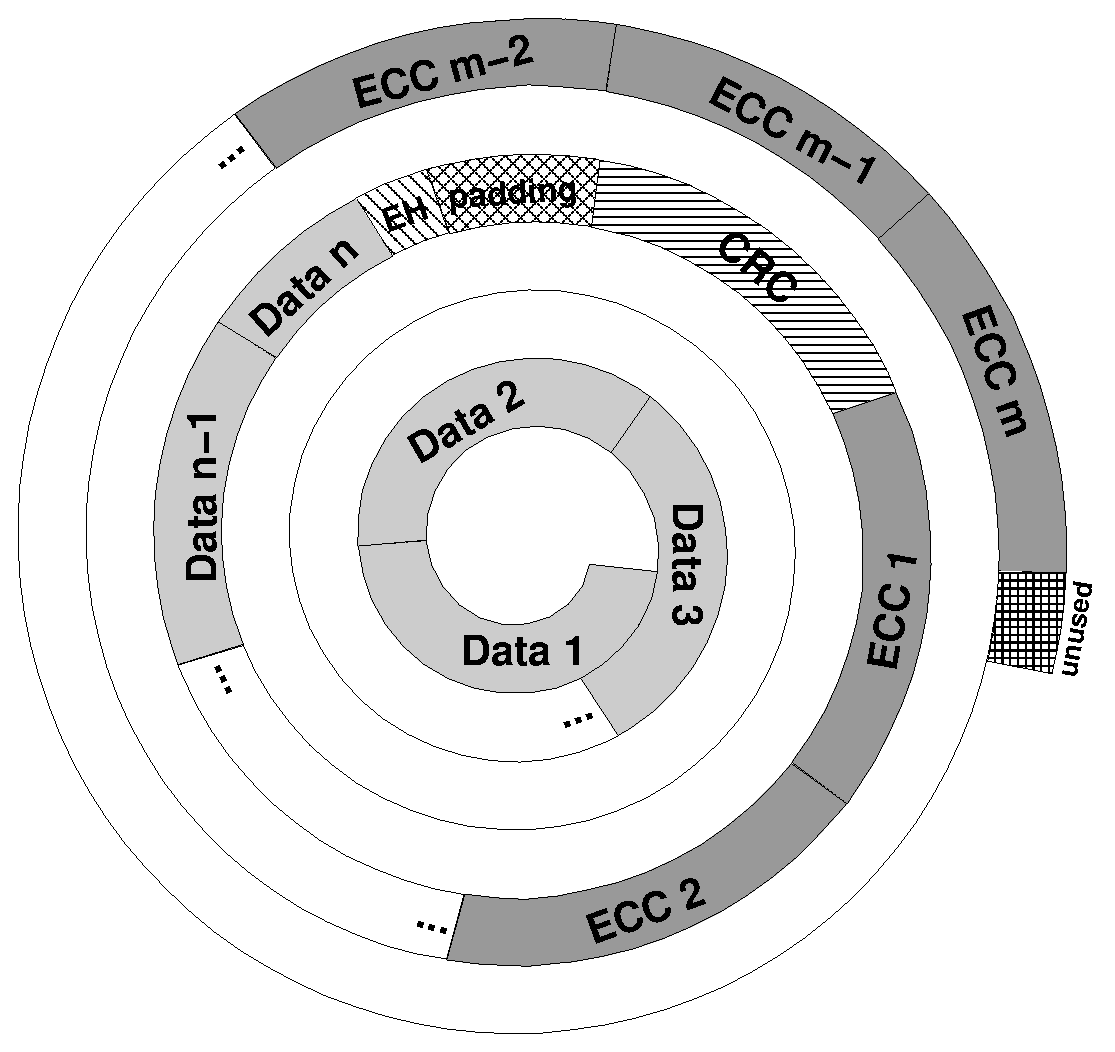
\includegraphics[width=10cm]{spiral-rs03.eps}
 \caption{Physical RS03 layout}
 \label{layout-phy}
 \end{center}
\end{figure}

This section describes the data format of the dvdisaster RS03 Reed-Solomon codec.
RS03 can store parity data either in a separate file or append it to the .iso
image on the same medium. In contrast to its predecessors RS03 is fully multi-threadable.
RS03  is expected to become the default codec soon after its introduction in 
dvdisaster 0.80.

\subsection{Physical layout}

Optical media are recorded as a single long spiral\footnote{Multiple layered
media contain one spiral for each physical layer, but are otherwise conceptually
identical.} of sectors which are indexed beginning with 0. 
The first sector lies at the innermost position of the spiral and 
numbering continues onward to the outside of the spiral.

Reed-Solomon encoding works best when errors are evenly distributed over
all ecc blocks. Therefore we must strive to spread our ecc blocks evenly over
the media surface. To facilitate such distribution, dvdisaster logically
divides the medium into 255 units which are called ``layers'' for historical reasons.
Figure \ref{layout-phy} illustrates how a medium is divided into $n$ data layers,
one CRC layer, and $m$ ecc layers, with $n+m+1 = 255$. Ecc blocks are comprised
by taking one byte from each layer as shown in fig. \ref{layout-logical} on 
the following page.
This distributes the ecc block reasonably good 
over the medium surface.

Layer size is measured in numbers of sectors which are 2048 bytes in size. All
255 layers have the same size. The data layers map exactly 
to the iso image which is to be protected by dvdisaster; 
e.g. the number and sequence of sectors in $Data_1,\ldots,Data_n$
is the same as in the iso image. Two extra sectors are appended to the ISO image
holding the ecc header ``EH''; these are logically treated as a part of the ISO image.
If the ISO image size plus the two EH headers is not an integer multiple
of the layer size, the last (n-th) data layer will be padded accordingly.  

The data layers are followed by a CRC layer. Each CRC layer sector contains a
data structure holding CRC32 checksums for the data sectors plus additional
parameters which were used during the RS03 encoding process.
The data and CRC layers are protected by the
Reed-Solomon parity which is stored in the remaining layers ($ECC_1,\ldots,ECC_m$).
Since the medium capacity is not necessarily an integer multiple of 255, some
unused sectors remain at the end of the medium. These are neither written nor
referenced in any way.

\smallskip

The RS03 data can be stored either directly on the medium or into a separate file.
Figure \ref{layout-phy} shows the first case where ecc data is embedded into the
image; this is also called a ``RS03 augmented ISO image'' in dvdisaster
terminology. 
In the other case a separate error correction file will be created containing
the sectors starting with the EH header. The following discussion is based
on the augmented image case; see section \ref{eccfile} for handling the
file based format.

\subsection{Logical layout}

\begin{figure}
 \begin{center}
 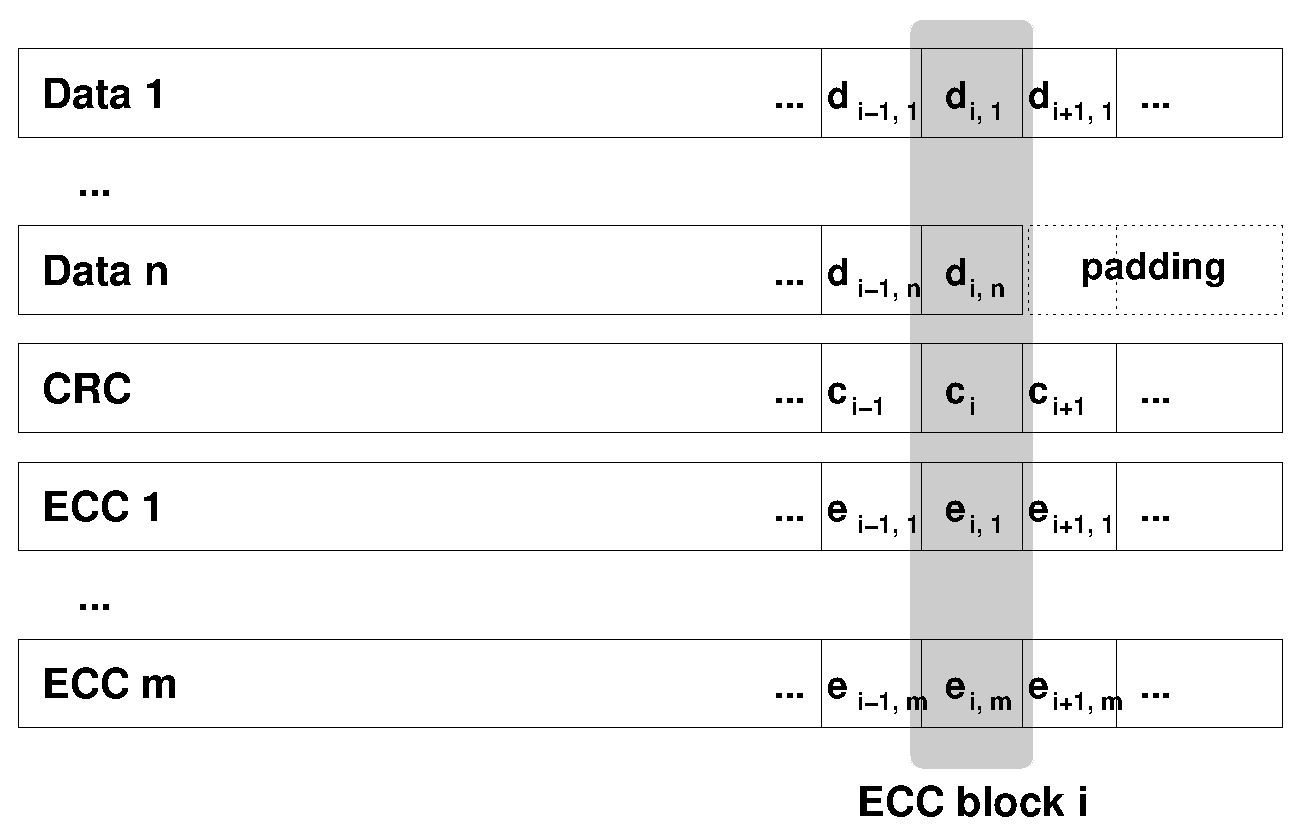
\includegraphics[width=\textwidth]{layer.eps}
 \caption{Logical RS03 layout}
 \label{layout-logical}
 \end{center}
\end{figure}


The relationship between layers and ecc blocks is stated again in the
logical view presented in figure \ref{layout-logical}. Here the 255 layers are
shown in stacked order. From each layer the $i-th$ byte corresponds to the
$i-th$ error correction block. The parity is calculated using $n$ data bytes
$d_{i,1},\ldots,d_{i,n}$ plus the crc byte $c_i$. The resulting $m$ roots of 
the completed Reed-Solomon code are then stored in the 
ecc bytes $e_{i,1},\ldots, e_{i,m}$. 

Since the input iso image plus the two EH sectors is usually not an integer 
multiple of the layer size, the last data layer $data_n$ may contain padding
sectors containing a special signature. The content of the padding sectors
is used in the ecc byte calculation and is written into the augmented image.

\subsection{Calculating the layout for encoding}

\begin{table}
 \begin{center}
 \begin{tabular}{|lrr|}
 \hline
 Medium type &  Maximum size & Layer size \\
 \hline
 CD & 359.424 & 1.409 \\
 DVD 1 layer & 2.295.104 & 9.000 \\
 DVD 2 layers & 4.171.712 & 16.359 \\
 BD 1 layer & 11.826.176 & 46.377 \\
 BD 2 layers & 23.652.352 & 92.754 \\
 \hline
 \end{tabular}
 \caption{Sector size parameters for several media types}
 \label{layout-size-table}
 \end{center}
\end{table}

When encoding with RS03 the layout of the augmented image is fully specified
by two values: the maximum medium size and the iso image size
(from now on, ``size'' always means ``number of 2048K sectors''). \bigskip

Media sizes are hard coded and taken from table \ref{layout-size-table}. Since we need to divide the medium into 255 layers, the layer size
is:
 
\[layer\ size = \left\lfloor\frac{medium\ size}{255}\right\rfloor\]

This allows us to compute the number of data layers needed to cover the iso image plus the ecc header:

\[data\ layers =  \left\lceil\frac{iso\ image\ size + 2}{layer\ size}\right\rceil\]

The number of padding sectors in the last data layer is:

\[padding\ sectors = layer\ size * data\ layers - iso\ image\ size - 2\]

For Reed-Solomon encoding, we will have to encode 

\[n\ data\ bytes = data\ layers + 1\]

and produce the following number of parity bytes:

\[m\ roots = 255 - n\ data\ bytes\]

The RS03 augmented image must fill the medium completely (except for the 
$medium\ size \bmod 255$ sectors  at the end). However for performance
reasons the maximum redundancy is capped to 200\%, or 170 roots. This means
that the ISO image must at least span the first 255-170=85 layers, otherwise
additional padding will be added to fill up the 85 data layers. This situation
is not reflected in the calculations and figure shown above.

\subsection{Re-calculating the layout from defective media}
\label{recover}

In order to recover a defective medium, the values of {\em layer size}
and {\em data layers} need to be determined. The RS03 format allows
for three heuristics with increasing complexity for learning about these
values:

\subsubsection{Using the Ecc Header}

All required information can be obtained from the data structures of the
Ecc Header which is described in appendix \ref{eh}. 
If ecc data is stored in a separate error correction
file, the first 4096 bytes of the ecc file yield the Ecc Header.
Otherwise, let $n$ be the size of the ISO file system which
can be obtained from the ISO file system master block. Then the 
Ecc Header is typically found in the RS03-augmented image at sectors $n,n+1$ 
or at $n+150,n+151$ (due to padding inserted by some popular CD-R  mastering
software). \smallskip

If the ISO file system master block is unreadable, the Ecc Header
can be identified by its characteristic signature and checksum. 
If the Ecc Header is encountered during reading of the defective medium 
it might be worthwhile to generate a tentative ISO master block in the image
file. This would speed up future processing of the image; however current
implementations of dvdisaster do not yet implement this feature.

\subsubsection{Using the CRC layer}

Each CRC layer sector contains a data structure which not only holds the
CRC32 checksums but also a copy of important parameters from the Ecc header
(see section \ref{crc} for details). CRC sectors can be easily recognized
by looking for their signature and checksum while scanning the medium image.
If dvdisaster finds a valid CRC sector and the Ecc header is defective,
a tentative Ecc header is written to the image to speed up further
operations on the image file.

However it should be noted that since all CRC sectors are stored 
consecutively on the medium, they can easily be wiped out by a large
defective region on the medium. Therefore, another heuristic exists
for learning about the RS03 layout.

\subsubsection{Evaluating the Reed-Solomon code}
\label{recover-rs}

If neither the Ecc Header nor any CRC sectors are readable
the RS03 layout can be determined by the following heuristic.

First, the medium size is determined from table \ref{layout-size-table}.
This is always possible as long as the drive will recognize the medium at all.
Since the layer size is $\left\lfloor\frac{medium\ size}{255}\right\rfloor$,
the location of the 255 layers on the medium is now known. The remaining task is to find
out the redundancy of the Reed-Solomon code, e.g. how many layers contain
roots for the RS code.

\bigskip

Taking the {\em i-th} sector from each layer will produce a valid error 
correction block, but with unknown redundancy. As RS03 will create redundancies 
using 8 to 170 roots, we employ a brute-force approach by evaluating
the Reed-Solomon code for $8..170$ roots. If the error correction
is successful for $n$ roots and the sector from layer {\em 255-1-n} yields
the CRC data structure, the correct number of roots has been found.

\medskip

In reality, not all 162 combinations of roots need to tested since additional
information can be exploited:

\begin{enumerate}
\item If the sector from layer {\em 255-1-n} is present/readable,
we do not need to test for $n$ roots any further: Encoding with $n$ roots would
have produced a CRC sector in this place.
\item If the number of erasures (as indicated by unreadable sectors) is higher
than $n$, we can trivially skip the RS decoding. We might have to test another
set of 255 sectors though if testing for all other numbers of roots fails as well.
\end{enumerate}

Criterion 1) should quickly narrow down the possible numbers of roots
in the average case, e.g. when enough redundancy is available for recovering the medium.
Worst case behaviour of trying each ecc block for 8..170 roots is likely to appear only
when the medium is unrecoverable, e.g. when more sectors are damaged than the 
Reed-Solomon code can correct.

\subsection{Contents of the CRC layer}
\label{crc}

Each sector of the CRC layer contains the data structure shown in
appendix \ref{crc-block}. Following the numbering from figure \ref{layout-logical},
CRC sector $c_i$ contains the CRC32 checksums for data sectors $d_{j,1},\ldots,d_{j,n}$
with $j = (i+1)\bmod\ layer\ size$. The purpose of this offset is to have
the error correction of ECC block $i$ recover the CRC checksum for the next 
ECC block $i+1$. In case of readable but corrupted sectors this will keep the
error correction in erasure mode and therefore save precious redundancy (the
RS code can recover twice as much errors when the location of defective data
is known). \medskip

Checksums for data sector $d_{j,k}$ are stored in array element
CrcBlock-$>$crc[k]. Unused array elements are set to zero.
The remaining contents of the CRC sector structure provide 
configuration and layout information; see appendix \ref{crc-block} for details.

\subsection{Encoding the ecc layers}

Encoding the error correction information
 requires reading and buffering of at least
255 sectors comprising the ecc block
(see fig. \ref{layout-logical} for a definition of the ecc block).
A possible encoding algorithm
might process each ecc block at a time. For each ecc block $i$
it would do the following: \smallskip

First, the $n$ data sectors $d_{i,1},\ldots,d_{i,n}$ of the ecc block
are read in. The CRC layer 
sector $c_i$ is initialized, filled in with checksums 
generated by processing the previous ecc block, and completed
by calculating its own checksum {\em selfCRC}. Unused portions of $c_i$
remain zero. Afterwards the
CRC32 checksums of $d_{i,1},\ldots,d_{i,n}$ are calculated
and stored away using the same buffering mechanism. Since the hand-over of
CRC checksums between ecc blocks is the only place where RS03 does 
not fully parallelize, data sector I/O and CRC32 caching needs to be 
carefully thought out in multithreaded implementations. \medskip


Once $d_{i,1},\ldots,d_{i,n}$ and $c_i$ have been prepared, 
2048 sets of a  RS(255,k) code (with $k=255-n-1$) are calculated by 
looping over the 2048 bytes of the ecc sectors. If $l$ denotes
a certain byte position between $0,\ldots,2047$ in the ecc block
sectors, then the {\em l-th} byte from $d_{i,1},\ldots,d_{i,n},c_i$
is retrieved and fed into the RS(255,k) encoder. The resulting
parity bytes $p_1,\ldots,p_m$ are stored in byte position $l$ of the
ecc layer sectors $e_{i,1},\ldots,e_{i,m}$. When all 2048 bytes
of the ecc block sectors have been processed the ecc layer sectors
can be written out; either into the error correction file or into
the RS03 augmented image. \medskip

The RS(255,k) encoder is the same for RS01, RS02 and RS03. See
appendix \ref{rs} for the parameters used in the encoder.

\subsection{Encoding as a separate error correction file}
\label{eccfile}

If the image size is too close to the medium capacity, not enough
space is left for augmenting the image with redundancy. dvdisaster
will refuse to augment images when there is insufficient space
for at least 8 roots. Creating images with less than 43 roots
(20\% of redundancy) will trigger a warning that the error correction
capacity may be too low. In those cases, storing the error correction
information in a separate file comes as an alternative.

\medskip

RS03 error correction files (``ecc files'')
contain the same error correction information
and layout as in the augmented image case, with the following differences:

\paragraph{Omittance of data padding sectors.} While the image format
shown in figures \ref{layout-phy} and \ref{layout-logical}
 may contain padding sectors between the ecc header and the CRC layer,
those sectors are not written into the ecc file.
The padding sectors are however required during encoding and
decoding, e.g. they need to be virtually created in memory 
when processing the respective ecc blocks. 
Therefore an ecc file providing {\em nroots} of redundancy
will contain {\em 2 + (nroots+1) * layer size} sectors.
Physically it will contain the ecc header, then the CRC layer 
and finally the {\em nroots} ecc layers. In contrast to the
augmented image case, the ecc header {\em is not part of an ecc
  block} and can therefore not be recovered
by the error correction. If the ecc header is lost in an ecc file,
its contents can be reconstructed from a still existing block
in the CRC layer and then be rewritten accordingly.

\paragraph{Freely chooseable redundancy.} In the augmented image case
the redundancy is always chosen to fill up the medium completely.
For ecc files the redundancy can be freely chosen by the user between
 8 roots (3.2\%) and 170 roots (200\%). Encoding with more than 170 roots
is technically possible, but run-time requirements get out of proportion;
hence the selectable redundancy is capped at 200\%.

\medskip

As a consequence of the variable redundancy the ecc file layout can only
be determined by looking at the ecc header or CRC sectors. The strategy
of experimentally evaluating the Reed-Solomon code (see sub 
section \ref{recover-rs}) however can not be applied to ecc files since
neither the size of the padding area nor the original size of the 
possibly truncated image and ecc files can be determined. \medskip

To see whether this is really a limiting factor we look
at the typical outcome of recovering a single file from a defective
medium:

\begin{itemize}
\item The ecc file is fully read, but random sectors are damaged.
\item The ecc file is truncated to the position of the first read error.
\end{itemize}

In both scenarios it is highly likely that at least one CRC sector survives
at the beginning of the file; in that case the error correction will not
only recover the image but also repair the ecc file into its original state.

\bigskip

Although this gives RS03 ecc files good chances to remain functional even
when being partly damaged, it is highly recommended to store ecc files 
only on media which are themself being protected by dvdisaster. 
ISO and UDF file systems
do not have sufficient redundancy for their meta data (e.g. directory
structures). If such meta data becomes unreadable a significant
number of files may become completely inaccessible. 
Please note that this is a
general weakness of file-based data protection and recovery: The
meta data is not part of any file and can therefore not be protected by
any error correction data put inside the file(s). 
\smallskip
This is the also the simple reason why we did not use tools like PAR2 
and developed dvdisaster instead; 
the image-based approach of dvdisaster protects
both files and meta data.


\newpage
\section{The RS02 codec}

This section describes the dvdisaster RS02 Reed-Solomon codec.
It was developed during the winter of 2005/2006 in order to facilitate
augmenting iso images directly with error correction data.

RS02 is based on the Reed-Solomon encoders and decoders 
introduced with RS01, but focuses exclusively on augmenting
iso images. The allocation of data sectors within an ecc block 
follows a similar scheme as in RS01. However the layout of the
parity bytes is vastly different between RS01 and RS02, as the codec must
cope with any parity sector being damaged or unreadable. 
Consequently a RS02 image can lose as many sectors as 
allowed by the redundancy of
the error correction data, and the lost sectors can be any
combination of data and parity sectors, as it is expected from
a Reed-Solomon scheme.

\smallskip

Unlike RS01, which will be completely superseded by RS03 soon,
the case of RS02 vs. RS03 still remains open, as both codecs
have their individual strengths. RS02 is slightly more space
efficient than RS03, so on CD media RS02 might provide
slightly more redundancy (typically one additional root) than RS03. 
This effect will be less
pronounced on larger media like DVD and BD. 
RS02 images can be augmented to an arbitrary size which may
be smaller than the maximum medium size, while RS03 requires
augmenting the image to the full medium size.
This might favour RS02 for working on images which are only
30\% or less of the medium size, as they can be encoded with
less than the maximum of 170 roots 
(the maximum redundancy requires lots of time to compute, producing
a three-fold redundancy which may not be needed in all cases). 
On the other hand RS03 will counter
the performance argument since it can encode at least 
20 times faster than RS02 on multi-core architectures, 
because RS02 encoding can not be parallelized. 
See the end of section \ref{rs01}  for a speed comparison of RS01 vs. RS03; 
RS01 and RS02 are very similar performance-wise.
Finally, the data layout of RS03 does not depend on interspersed
ecc headers which gives it a better robustness over RS02;
see subsection \ref{layout-logical-two} for details.

\subsection{Physical layout}

\begin{figure}
 \begin{center}
 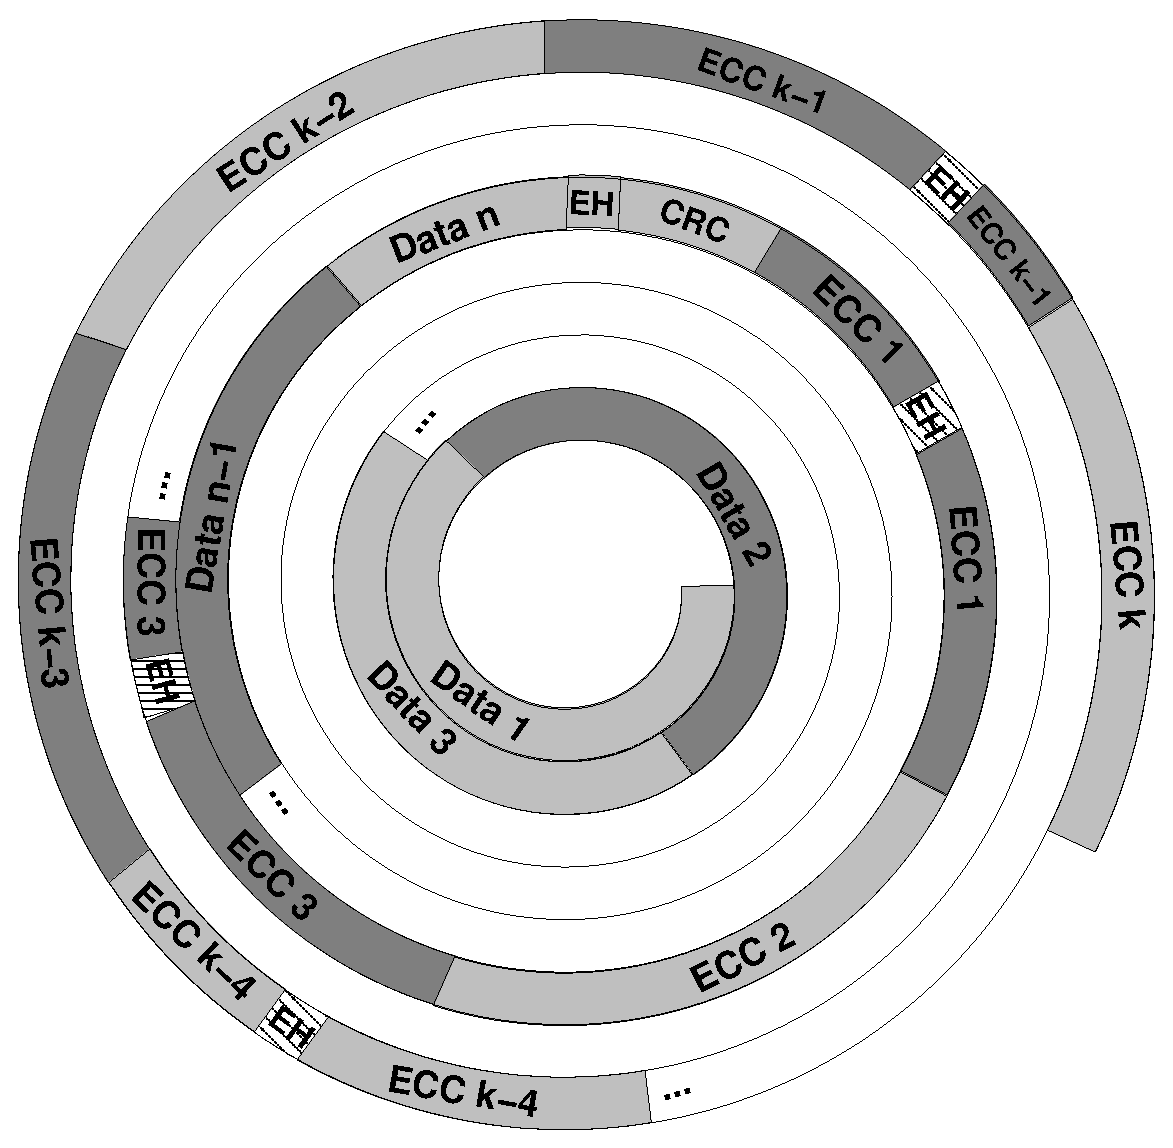
\includegraphics[width=10cm]{spiral-rs02.eps}
 \caption{Physical RS02 layout}
 \label{layout-phy-two}
 \end{center}
\end{figure}

RS02 must be applied to the .iso image before it is written to
the medium. Additional sectors are appended to the .iso image 
containing the parity data. The data structures of the .iso image
are not changed to reflect the new image size, so the original
part of the augmented .iso image remains untouched. The parity
sectors can be removed from the augmented image by simply 
truncating the .iso image to its original sector size; the resulting
image file will have the same contents as prior to the augmentation.
As a side effect, the parity data is invisible to applications reading
the medium at the filesystem level, including most hardware media
players. If you find a player which gets confused by media containing
RS02 (or RS03) parity, please consider telling the dvdisaster project about it. As of this writing,
not a single device has been reported to run into problems with
the RS02 data scheme. The RS02 augmented image might conflict with
optical media writing software, though. If the writing software
decides the image length by looking at the iso filesystem structures,
the parity data portion of the image might not be written to the medium.
Most current writing programs do however measure the .iso image by examining
its file size, and will transfer the parity data correctly. To be sure you
should follow the steps described under ``Testing image compatibility''
at the dvdisaster site (\url{http://dvdisaster.net/en/howtos92.html}) once
before using each version of your optical media authoring software.

Like the other dvdisaster codecs, RS02 is based on a  RS(255,k) Reed-Solomon code
with each ecc block being comprised of $n$ data bytes and $k$ parity bytes, and
$n+k=255$. The $n$ data bytes comprise the .iso image which will be
written to the medium, and the additional ecc header and CRC checksums added
by dvdisaster. Reed-Solomon encoding works best when errors are
distributed evenly over all ecc blocks. Therefore we must strive to distribute
the ecc blocks evenly over the medium surface. To facilitate such mapping,
dvdisaster logically divides the medium into 255 logical units which are called
``layers'' for historical reasons. 
Figure \ref{layout-phy-two} shows how the medium is divided into $n$ data layers
and $k$ ecc layers, with $n + k = 255$. Ecc blocks are
created by taking on byte from each layer as shown in fig. \ref{layout-logical-two}
on the following page. This distributes the ecc block reasonably good over
the medium surface. 
All layers have the same length in bytes, with the possible exception of
data layer $n$. As the .iso image size plus the size of one ecc header and the CRC data
is usually not a multiple of the layer size, the $n$-th data layer may be shorter
than the layer size and considered to be filled up with a virtual zero padding. 
The zero padding is not written out to the augmented image (note that data layer $n$
is intentionally drawn shorter in fig. \ref{layout-phy-two}), but it is used in the
calculation of the respective parity bytes.

\newpage

\subsection{Logical layout}
\label{sec-layout-logical-two}

\begin{figure}
 \begin{center}
 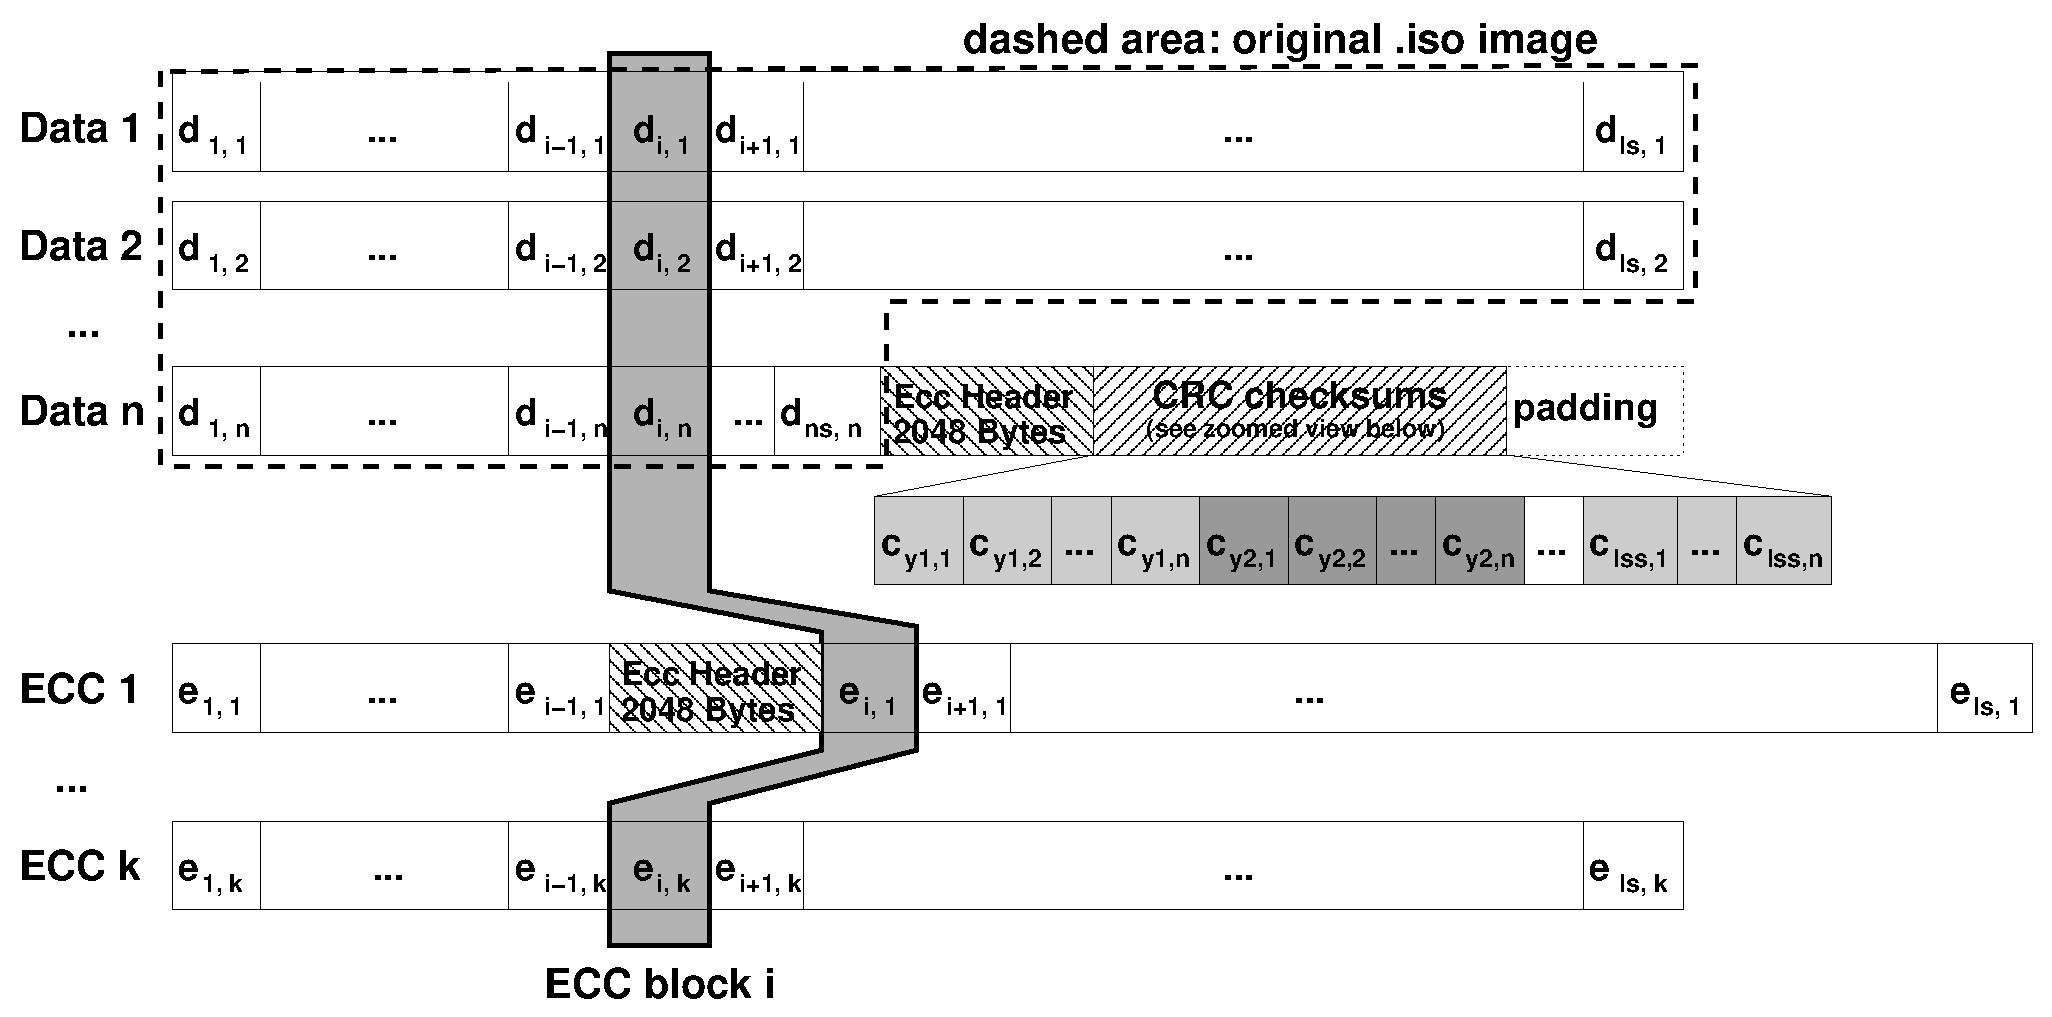
\includegraphics[width=\textwidth]{rs02-layout.eps}
 \caption{Logical RS02 layout}
 \label{layout-logical-two}
 \end{center}
\end{figure}

The data layout in the augmented image is shown in figure \ref{layout-logical-two}.
Note that in this figure the data is byte-indexed; e.g. $d_{1,1}$ denotes the
first data byte in the augmented image. Each layer has a length of
$ls$ bytes, with the exception of data layer $n$ which may be shortened (see subsection \ref{calc-two} for an exact calculation of its size). 
Some ecc layers my be interleaved with redundant copies of the ecc header. 
The ecc header size is not included in the respective ecc layer size.

\paragraph{Data layers.} A data layer index $d_{i,j}$ refers to the $i$-th byte in the $j$-th data layer.
The $n$ data layers are mapped in a linear fashion to the original iso image.
$d_{1,1}$ maps to the first .iso image byte, and $d_{ns,n}$ maps to the last .iso image
byte ($ns$ is the number of remaining iso image bytes in the $n$-th data layer). 

The last data layer is special because it does not only contain the rest of the iso image,
but also the ecc header and the CRC checksums. These extensions 
are logically treated as a part of the iso image; their contents are used in the
ecc data calculation and are therefore protected by the ecc data.
The ecc header follows immediately after byte $d_{ns,n}$ and is 4096 bytes long.
Its format is described in appendix \ref{eh}. For RS02, only the data fields
marked with ``all'' or ``RS02'' are relevant; all other fields should be set to zero.

Data layer $n$ does also contain the CRC32 checksums of each data sector
upto the ecc header. If the .iso image contains $s$ sectors, 
then the CRC field contains $4s$ bytes, rounded up
to the nearest multiple of 2048. 
CRC32 checksums are calculated over a whole CD sector comprising 2048 bytes.
Let $c_{y,j}$ be the 4-byte checksum of the $y$-th sector in the $j$-th layer
and $lss$ be the number of sectors in each layer.
Then $c_{y,j}$ = CRC32($d_{2048*y,j}$, $d_{2048*y+1,j}$, \dots, $d_{2048*y+2047,j}$).  
 
$y_1$ is usually not the first sector in the layer, but a later sector.
In general, $y_i$ = $(i+offset)$ mod $lss$. The offset is introduced to restore
the CRC32 sums of ecc block $i+1$ during the correction of ecc block $i$.
This helps if the data portion of the image is corrupted with wrong byte values and
the sectors containing the CRC32 sums have been lost. 
The error correction will start at the ecc block $i$ which is determined
by the offset, and whose CRC32 checksums are stored in the ecc header (at least one
ecc header will be recovered before any error correction can begin). Correcting
ecc block $i$ will recover the CRC32 checksums for ecc block $i+1$ in the image
(and possibly some more in advance, as less than 2048 bytes are required for
one set of checksums). This makes it possible to detect corrupted bytes by the
checksums and flag them as erasures which effectively doubles the error correction
capabilities of the Reed-Solomon code.

\paragraph{Ecc layers.} For an image augmented with $k$ roots, the parity bytes
will be spread over $k$ ecc layers. In order to calculate the first ecc block,
bytes $d_{1,1}$ to $d_{1,n}$ are taken from the $n$ data layers. The RS(255,k) code
is calculated (see appendix \ref{rs} for its parameters) and the resulting $k$
parity bytes $e_{1,1}$ to $e_{1,k}$ are stored in the $k$ ecc layers. 
The next ecc blocks are calculated and stored accordingly; ecc block $i$ 
is marked grey in the figure.
Care must be taken to honour the non-linear mapping of
ecc layer bytes as the ecc area is interleaved with 20-40 copies of the ecc header.
The ecc header copies are placed at sector addresses whose numbers 
are large powers of two. This makes it possible to heuristically search for them
during the decoding boot-strap process 
when no other information (image size, layer size, etc.) is yet available.
See section \ref{search-two} on the search heuristics and section \ref{addressing-two}
on calculating ecc bytes positions from the non-linear mapping. 

\subsection{Calculating the image layout for encoding}

The image layout can be either computed automatically to fill up
the medium as much as possible, or by user selected criteria such
as a maximum image size or a specified redundancy.

\subsubsection{Automatic layout calculation}
\label{calc-two}

The only available inputs to automatic layout detection are
the .iso image size and a table of maximum media sizes (see
tab. \ref{layout-size-table} in the RS03 section for the
respective values). From the media size table the smallest
possible medium  is chosen which can contain the .iso image.
In some border cases, with e.g. the .iso image being only
100 sectors smaller than the medium capacity, the automatic
layout calculation will fail later due to insufficient space
on the medium. In such cases, the user must decide between
choosing the next larger medium size or splitting the image
contents onto two media by himself (splitting a 700MiB CD image 
onto two CDs may be better than writing it to a DVD).

\smallskip

From now on, all calculations are given in numbers of 2048K 
sectors or sectors addresses
unless noted otherwise. The number of sectors required for the
CRC checksums can be directly computed from the .iso image size:

\[
crc\; sectors = \left\lceil\frac{4 * iso\; image\; sectors}{2048}\right\rceil
\]

The total accumulated size of all data layers is the sum of the
.iso image size, the number of crc sectors and the two sectors required
for the ecc header. Since these sectors are protected by the parity,
they are called {\em protected sectors}:

\[protected\; sectors = iso\; image\; size + 2 + crc\; sectors\]
 
These calculations also produce two important sector addresses within
the augmented image:

\begin{itemize}
\item The sector with address {\em iso image size} marks the location
of the ecc header; and
\item The sector at address $iso\; image\; size + 2$ marks the beginning
of the CRC checksum data.
\end{itemize}

The next step is to partition the {\em protected sectors} and the remaining
medium space into an optimal layer size. It is carried out iteratively.

\smallskip

For an approximate start, we determine the free space on the medium:

\[free\; space = medium\; capacity - protected\; sectors\]

and estimate a preliminary value for the number of roots and data layers:

\[k\; roots = min\left(170, \quad\left\lfloor\frac{255 * free\; space}{medium\; capacity}\right\rfloor\right)\]

\[n\; data = 255 - k\; roots\]

The maximum number of roots is capped at 170 which is approximately a three-fold
redundancy. Larger values would get too computationally expensive.

\smallskip

The preliminary layer size is then:

\[preliminary\; layer\; size = \left\lceil\frac{protected\; sectors}{n\; data}\right\rceil\]

and the expected size of the parity layers is:

\[preliminary\; ecc\; size = k\; roots * preliminary\; layer\; size\]

\smallskip

% TODO: implement in codec
\begin{comment}

From these values we iteratively compute a $2^p$ which has about 20-40 multiples
in the {\em preliminary ecc size} address space. This value will be used
for interleaving the ecc header copies with the ecc layers:

\smallskip

{\tt
p := 5

while($\frac{preliminary\;ecc\;size}{2^p} > 40$)

\quad p := p + 1}  
\end{comment}

From these values we compute a $2^p$ which has about 20-40 multiples
in the {\em preliminary ecc size} address space. This value will be used
for interleaving the ecc header copies with the ecc layers:

\[ p = \left\lceil log_2\; \frac{preliminary\;ecc\;size}{40} \right\rceil \]

%\[ p = \left\lceil \frac{log\; \frac{preliminary\;ecc\;size}{40}}{log\; 2} \right\rceil \]


\smallskip

Now the chosen values might be actually too big since we haven't taken
the ecc header copies into account. 
So the final task is to add up the number pf parity sectors and ecc header
copies. If these fit into the free medium space, we are done; otherwise
the calculations are done again with one root less.

\newpage

\bigskip

while($n\; roots > 7$)

\smallskip

\quad $layer\; size := \left\lceil\frac{protected\; sectors}{n\; data}\right\rceil$

\smallskip

\quad $ecc\; size := n\; roots * layer\; size$

\smallskip

\quad $first\; ecc\; header\; repeat\; addr := \left\lceil\frac{protected\; sectors}{2^p}\right\rceil * 2^p$ 

\smallskip

\quad $space\; for\; interleaved\; sectors := protected\; sectors + ecc\; size - first\; ecc\; header\; repeat\; addr$

\smallskip

\quad $number\; of\; ecc\; copies := \left\lfloor\frac{space\; for\; interleaved\; sectors}{2^p - 2}\right\rfloor + 1$

\smallskip

\quad $total\; added\; sectors := 2 + crc\; sectors + ecc\; size + 2 * number\; of\; ecc\; copies$

\medskip

\quad If $iso\; image\; sectors + total\; added\; sectors < medium\; size$,
we have a valid layout: STOP.

\smallskip

\quad Otherwise, set $n\; roots := n\; roots - 1$ and $n\; data := 255 - n\; roots$
and do another iteration. 

\medskip

The iteration will either terminate with a valid layout or fail when
$n\; roots$ drops below the minimum redundancy of 8 roots. 

\subsubsection{Layout calculation by user selected criteria}

The user has several means of specifying a certain redundancy:

\paragraph{Specifying the maximum number of sectors for the augmented image.}

This case is simply handled by setting {\em medium capacity} to the user
selected sector size rather than using the maximum medium size from the
built-in table. Afterwards, calculations continue as described in
section \ref{calc-two}.

\paragraph{Specifying the number of roots to use.}

In this case we can skip the calculations for {\em free space} and
{\em k roots} as described in section \ref{calc-two}, and instead
set {\em k roots} directly to the user selected value. Then the
layout calculation proceeds as usual. 

\paragraph{Specifying the percentage of redundancy to use.}

For a given number of {\em k roots}, the resulting redundancy in percent is:

\[\frac{k\; roots \cdot 100}{255 - k\; roots}\]

Pick a suitable value for {\em k roots} so that the user selected value
is met or slightly exceeded. Proceed with the given number of roots
as described in the previous paragraph.

\subsubsection{Layout calculation from ecc header information}
\label{recalc-layout-header-two}

In a given ecc header struct {\em eh}, the number of sectors in the .iso
image is recorded as \mbox{\em eh-$>$sectors} 
and the number of roots is contained in \mbox{\em eh-$>$eccBytes}.
Calculation of the layout is done as shown in section \ref{calc-two}, 
with the exception of omitting the calculation for {\em free space} and
setting {\em k roots} directly to  \mbox{\em eh-$>$eccBytes}.

\subsection{Automatic layout calculation example}
\label{example-two}

Let's assume we are going to encode an .iso image of 295.000 sectors.
This is well below the CD medium capacity of 359.424 sectors, so we
start with:

\smallskip

$medium\; capacity = 359.424\; sectors$

$iso\; image\; size = 295.000\; sectors$

\medskip

The number of CRC sectors will be:

\smallskip

$crc\; sectors = \left\lfloor\frac{4 * 295.000}{2.048}\right\rfloor = 577\; sectors$

\medskip

The total size of all data layers is:

$protected\; sectors = 295.000 + 2 + 577 = 295.579\; sectors$

\bigskip

The next step is creating some preliminary starting values:

\smallskip

$free\; space = 359.424 - 295.579 = 63.845\; sectors$

\smallskip

$k\; roots = min\left(170, \left\lfloor\frac{255* 63.845}{359.424}\right\rfloor\right) = min(170, 45) = 45\; roots\; (or\; layers)$

\smallskip

$n\; data = 255 - 45 = 210\; layers$

\bigskip

Now some more preliminary values can be computed:

\smallskip

$preliminary\; layer\; size = \left\lceil\frac{295.579}{210}\right\rceil = 1.408\; sectors$

\smallskip

$preliminary\; ecc\; size = 45 * 1.408 = 63.360\; sectors$

\bigskip

Finally, we compute $p = 11$ since $\frac{63360}{2^{11}} = 30,9$.

\bigskip

Now the chosen values must be verified to produce a layout which is
still smaller than the image size. We compute (the first two values are already known):

\medskip

$layer\; size = \left\lceil\frac{295.579}{210}\right\rceil = 1.408\; sectors$

\smallskip

$ecc\; size = 45 * 1.408 = 63.360\; sectors$

\smallskip

$first\; ecc\; header\; repeat\; addr = \left\lceil\frac{295.579}{2048}\right\rceil * 2048 = 296.960$

\smallskip 

$space\; for\; interleaved\; sectors = 295.579 + 63.360 - 296.960 = 61.979\; sectors$

\smallskip

$number\; of\; ecc\; copies = \left\lfloor\frac{61.979}{2048-2}\right\rfloor + 1 = 31\; header\; repeats$

\smallskip

$total\; added\; sectors = 2 + 577 + 63.360 + 2 * 31 = 64.001\; sectors$

\medskip

This layout will generate an augmented image containing
$295.000 + 64.001 = 359.001$ sectors which is 
less than the medium capacity of 359.424 sectors
and therefore accepted.

\subsection{Re-calculating the layout from defective media}
\label{search-two}

In order to recover a defective medium, at least one ecc header must
remain readable and be located by the following heuristic. This
is a major difference to RS03, which has more and different means
for bootstrapping the recovery (see section \ref{recover} for details).
Once one ecc header has been recovered, the ecc data layout can be
calculated as described in section \ref{recalc-layout-header-two}.
From this point, the error correction is done using the parameters
and data described in section \ref{encoding-two}.

\smallskip

If the medium is not damaged or only slightly damaged, the following
short cut might work: The size of the .iso image can be determined
from the iso file system header. Then the ecc header immediately
following the .iso image part of the augmented image is either
located at sector number $iso\;image\;size$ or $iso\;image\;size + 150$.
The latter case arises because some popular CD authoring software
appends 150 padding sectors to any .iso image it creates. 

\smallskip

If the short cut does not work due to the required sectors being damaged,
the following strategy is employed. The size of the augmented image
can always be determined; it can either be queried from the drive or
it is the file size of a file-based image. Then apply the following
algorithm:

\bigskip

$p = \left\lfloor log_2(image\; size)\right\rfloor$

while $p > 32$

\quad $pos = \left\lfloor\frac{image\; size}{2^p}\right\rfloor \cdot 2^p$

\smallskip

\quad while $pos > 0$

\qquad if {\em sector at pos} is a valid ecc header: STOP.

\qquad if {\em sector at pos} is unreadable, set $pos := pos - 2^p$ .

\hspace*{13mm} Continue with inner while loop.

\qquad if {\em sector at pos} is readable and not a ecc header, set $p := p -1$ .

\hspace*{13mm} Continue with outer while loop.

\bigskip

In order to test for a valid ecc header, check that {\em ec-$>$cookie}
equals the 16-byte string ``*dvdisaster*RS02''. Then check that the
CRC32 sum of the ecc header matches the value recorded in {\em eh-$>$selfCRC},
with {\em eh-$>$selfCRC} set to the byte sequence 0x47,0x50,0x4c,0x00
for the purpose of calculating the CRC32 sum.

\medskip

Please notice that during testing of the sectors at multiples of $2^{(p-1)}$,
all sectors previously tested for $2^p$ will be examined again. It is therefore
highly recommended to cache results from previous iterations of the outer
while loop, especially when reading sectors from the optical medium.



\subsection{Sector addressing and initialization scheme}
\label{addressing-two}

For encoding and decoding purposes it is required to retrieve the
{\em i-th} sector from the {\em j-th} data or ecc layers, e.g. to calculate
the corresponding sector number in the augmented image. 
The reverse calculation is also needed, e.g. to calculate the
corresponding layer and sector index for a given sector number
in the augmented image.

\smallskip

Bear in mind that as shown in figure \ref{layout-logical-two}, an augmented image 
is divided into two logical parts. There is a data area containing 
the .iso image contents, the first ecc header and the CRC checksums.
The data area is protected by the parity in the ecc area, which contains
the parity data interleaved with copies of the ecc header. 

\smallskip

In order to carry out the calculations described below, the following
values from the layout calculation (see section \ref{calc-two} are required:

\bigskip

\begin{tabular}{lp{10cm}}
{\em protected sectors} & the size of the data part in sectors \\
{\em layer size} & the number of sectors per layer \\
{\em $2^p$} & the modulo value for locating ecc header copies \\
\end{tabular}

\paragraph{Converting (layer, sector index) pairs into image sector numbers.}

The {\em i-th} sector of data layer {\em j} has the following address $s$ in the image:

\[s = j \cdot layer\; size + i\]

If $s >= protected\; sectors$, $s$ is a padding sector which must not be read 
from the image file, but created in memory (see the paragraph on initialization below).

\bigskip

To calculate the sector address $es$ of the {\em i-th} sector from the {\em j-th} 
ecc layer, the non-linear mapping of the ecc sectors has to be taken into account.
The index of the first interleaved ecc header is:

\[ first\; interleaved = \left\lceil\frac{protected\; sectors}{2^p}\right\rceil \cdot 2^p\]

Since {\em protected sectors} is equal to the address of the first ecc sector in the image,
the amount of ecc sectors before the first interleaved ecc header is:

\[ base\; ecc\; sectors = first\; interleaved - protected\; sectors\]

The ecc sector we are looking for would have the following index if ecc
sectors were linearly mapped:

\[ ecc\; index = j \cdot layer\; size + i\]

If {\em ecc index $<$ base ecc sectors}, $es$ = {\em protected sectors} + {\em ecc index}.
Otherwise, the non-linear mapping must be taken into account. The number of interleaved
ecc headers before the (currently unknown) sector position $es$ is:

\[ interleaved\; headers = \left\lfloor\frac{ecc\; index - base\; ecc\; sectors}{2^p - 2}\right\rfloor \]

Therfore the position of the ecc sector in the augmented image is:

\[ es = protected\; sectors + ecc\; index + 2 \cdot interleaved\; headers + 2 \] 

\paragraph{Example.} To continue the example from section \ref{example-two}, the
position of the 17th ecc sector in the 3rd ecc layer shall be computed. The relevant
layout values are:

\smallskip

\begin{center}
\begin{tabular}{rll}
{\em protected sectors} & = & 295.579 \\
{\em layer size} & = & 1.408 \\
{\em $2^p$} & = & 2.048 \\
\end{tabular}
\end{center}

The first interleaved ecc header is at position:

\[ first\; interleaved = \left\lceil\frac{295.579}{2.048}\right\rceil \cdot 2.048 = 296.960 \]

Before the first interleaved ecc header,

\[ base\; ecc\; sectors = 296.960 - 295.579 = 1.381 \]

ecc sectors have been stored. The linear index of the sought ecc sector is:

\[ ecc\; index = 3 \cdot 1.408 + 17 = 4.241 \]

Since 4.241 $\ge$ 1.381, the embedded ecc headers must be taken into account. There are

\[ interleaved \; headers = \left\lfloor\frac{4.241 - 1.381}{2.048-2}\right\rfloor = 1 \]

interleaved ecc headers, each containing 2 physical sectors. Therefore the position
of the sought ecc sector in the image is:

\[ es = 295.579 + 4.241 + 2 + 2 = 299.824 \]

\bigskip

{\bf Converting image sector numbers into (layer, sector index pairs).}

\smallskip

If the sector number $s$ $<$ {\em protected sectors}, the sector will map to the data part
as follows:

\[layer = \left\lfloor s\; /\; layer\;size \right\rfloor\]
\[i = s \bmod layer\;size\]

Otherwise, the mapping to the ecc part is calculated as follows. The index of the first interleaved ecc header is:

\[ first\; interleaved = \left\lceil\frac{protected\; sectors}{2^p}\right\rceil \cdot 2^p\]

If $s\; mod\; 2^p \le 1$, the sector maps to the {\em n-th} interleaved ecc header, with:

\[n = \left\lfloor\frac{s - first\; interleaved}{2^p}\right\rfloor\] 

If $s < first\; interleaved$, the sector is an ecc parity sector with the following mapping:

\[ layer = \left\lfloor(s - protected\; sectors)\; /\; layer\; size\right\rfloor\]
\[ i = (s - protected\; sectors)\; mod\; layer\;size\]

If $s \ge first\; interleaved$, the mapping of the ecc parity sector is calculated as follows:

The amount of ecc sectors before the first interleaved ecc header is:

\[ base\; ecc\; sectors = first\; interleaved - protected\; sectors\]

The number of interleaved ecc headers before sector $s$ is:

\[ interleaved\; headers = \left\lfloor\frac{s - first\; interleaved - 2}{2^p}\right\rfloor \]

If ecc sectors were mapped linearly, then $s$ had the linear index:

\[ ecc\; index = s - protected\; sectors - 2 \cdot interleaved\; headers - 2\]

Finally, this means that $s$ maps to the following parity sector:

\[ layer = \left\lfloor ecc\; index\; /\; layer\; size\right\rfloor \]
\[ i = ecc\;index \bmod layer\; size \]

\paragraph{Padding sectors.} Let {\em iso image size} be the size of the
.iso image prior to augmenting it with error correction data. In order
to augment the image with error correction sectors, the following
sectors are treated as padding sectors which are filled with zeroes:

\begin{itemize}
\item All sectors $s$ $>$ {\em protected sectors}.
\item The first ecc header (sectors $iso\; image\; size$ and $iso\; image\; size+1$).
\end{itemize}
 
The first ecc header sectors must be treated as padding to break a circular
dependency with the parity bytes; as the ecc header contains a md5 sum over
all parity bytes, it can not be used as input for the parity generation.

\subsection{Encoding the checksums}
\label{crc-two}

For each sector of the .iso image a CRC32 checksum is calculated and stored in the
data part of the augmented image (see fig. \ref{layout-logical-two}). By using the
conventions of section \ref{sec-layout-logical-two}, let $d_{i,j}$ be the $i$-th byte
of the $j$-th data layer and $c(y,j)$ the 4-byte checksum of the $y$-th sector
in the $j$-th data layer. Then $c(y,j)$ = CRC32($d_{2048*y,j}$, $d_{2048*y+1,j}$, \dots, $d_{2048*y+2047,j}$).  

\smallskip

Let $first\; layer\; crc\; idx = (iso\; image\; size + 2) \bmod layer\; size$. 

$n$ is the number of data layers.

\smallskip

A total of $\left\lceil\frac{iso\; image\; size}{512}\right\rceil$ sectors holding the
CRC32 checksums must be generated. The checksums are sorted by the layer sector $y$ first, 
then by layer number $i$. So for each layer sector $y$, there is a block of $n$ checksums generated,
and there are $layer\; size$ blocks of checksums total. Checksum generation does not start with
layer sector $0$, but rather with layer sector $first\; layer\; crc\; idx$. Subsequent blocks
are generated in ascending layer sector order {\em modulo layer size} so that all
{\em layer  size} layer sector positions are eventually covered. 
This scheme produces the following
sequence of checksums: 

\medskip

\begin{tabular}{l}
$c((first\; layer\; crc\; idx + 1) \bmod layer\; size, \quad 1)$\\
$c((first\; layer\; crc\; idx + 1) \bmod layer\; size, \quad 2)$\\
\dots\\
$c((first\; layer\; crc\; idx + 1) \bmod layer\; size, \quad n)$\\
\hline
\end{tabular}

\begin{tabular}{l}

$c((first\; layer\; crc\; idx + 2) \bmod layer\; size, \quad 1)$\\
$c((first\; layer\; crc\; idx + 2) \bmod layer\; size, \quad 2)$\\
\dots\\
$c((first\; layer\; crc\; idx + 2) \bmod layer\; size, \quad n)$\\
\hline
\end{tabular}

\begin{tabular}{l}
\dots\hspace*{81mm}\\[1mm]
\hline
\end{tabular}

\begin{tabular}{l}
$c((first\; layer\; crc\; idx + layer\; size -1) \bmod layer\; size, \quad 1)$\\
$c((first\; layer\; crc\; idx + layer\; size -1) \bmod layer\; size, \quad 2)$\\
\dots\\
$c(first\; layer\; crc\; idx \bmod layer\; size, \quad n-1^*)$\\
\hline
\end{tabular}

\begin{tabular}{l}
$c(first\; layer\; crc\; idx \bmod layer\; size, \quad 1)$\\
$c(first\; layer\; crc\; idx \bmod layer\; size, \quad 2)$\\
\dots\\
$c(first\; layer\; crc\; idx \bmod layer\; size, \quad n-1^*)$\\
\end{tabular}

\bigskip

$^{*)}$ The last sectors of each data layer may be padding sectors. For those padding
sectors, {\em no} CRC32 checksums are generated and stored (e.g. the number of
generated checksums is always exactly {\em iso image size}).

Since {\em iso image size} is usually not a multiple of 512, the last sector in
the data part may only be partially filled with checksum data. The remaining
bytes of this sector must be filled with the repeated byte sequence
0x47,0x50,0x4c,0x00 which is the ASCII string representation of the text ``GPL''.

\smallskip

A copy of the CRC32 sums for the layer sectors at position ($first\; layer\; crc\; idx \bmod layer\; size$)
is stored in the ecc header, starting there at byte position 2048. This has the advantage that
the CRC checksums are already available for the {\em first layer crc}-th sectors
of data layers $1,\ldots,n$. Any corrupted bytes in those sectors are
detected by the CRC32 and can be handled by the error correction in erasure mode,
saving precious parity bytes. When the error correction has restored all sectors
of the {\em first layer crc}-th ecc block, note that the {\em first layer crc}-th
sector of data layer $n$ will contain the CRC32 checksums for the data sectors 
in the next ecc block ({\em first layer crc + 1}). Therefore the layout is robust
against loss of CRC sectors as they are restored by the error correction just
before they are actually needed.

\subsection{Encoding the ecc layers}
\label{encoding-two}

Encoding the ecc layers requires the following steps:

\medskip

First the image must be examined whether it does already contain
augmented ecc data (either RS02 or RS03). If ecc data is found, the
image must be stripped to the original size of the .iso image. 
Nesting ecc data is not supported by the current codecs and it
might derail the heuristics for detecting the augmented data
properly. From a technical point, nesting ecc data does not
make sense either.

\medskip

Next the image must be checked for missing sectors, and be rejected
if it is incomplete. Producing and
writing images with missing sectors to a medium is
confusing to the user as dvdisaster will always report 
the medium as partially readable even though it does not contain
any physical defects. Also the error correction will never
succeed for such media as it is just restoring the sector
in its missing  state. 
During the check for missing sectors the CRC32 checksums 
of each sector can be computed as described in section \ref{crc-two} and, 
after writing a placeholder for the first ecc header, be appended to the image.
Also, the MD5 sum of the .iso image can be calculated at this time and
kept for insertion into the ecc header field {\em ec-$>$mediumSum}.
As another step of preparation, enough space should be appended
to the image to store the ecc layer sectors. This makes sure
that the encoder does not run out of disk space during
its potentially lenghty work, and minimizes the impact of
fragmentation due to random writes into the appended 
image area under most file systems.

\medskip

Finally, the error correction information needs to be encoded.
Please refer to fig. \ref{layout-logical-two} on the location
of the bytes comprising an error correction block.
Although the ecc blocks could be encoded by a byte-wise scheme, 
a possible encoding algorithm would preferably buffer at least the 
255 sectors holding the required data for 2048 subsequent ecc
blocks, and process those in bulk. From the first $n$ data layers,
the required bytes are retrieved and fed into the RS(255,k)
Reed-Solomon encoder, with $k = 255 -n$. The RS(255,k) encoder 
is the same for RS01, RS02 and RS03. See
appendix \ref{rs} for the parameters used in the encoder.
 
Please refer to
the previous section on information about zeroed-out and
zero-padded data sectors. The resulting $k$ parity bytes
are distributed into the $k$ ecc layers. When writing out
the ecc data into the image, free gaps must be left for
the interleaved ecc headers; see section
\ref{addressing-two} for information on calculating the
interleaved ecc header positions. At this time, the MD5
sums of each ecc layer can be updated incrementally. 

\medskip

When all parity sectors have been calculated, the ecc headers
can be completed by filling in their {\em eh-$>$eccSum} field.
This field contains the MD5 sum calculated over the MD5 sums
over each of the $k$ ecc layers. In contrast to a single MD5
sum spanning the ecc layers in a linear fashion, this
approach allows for an incremental calculation of the MD5 sum
while the ecc data is generated and written out. 


\newpage
\section{The RS01 codec}
\label{rs01}
This section describes the dvdisaster RS01 Reed-Solomon codec. 
It was conceived during the summer of 2004 for creating 
error correction files in the first dvdisaster versions.
At this time, CD media was still predominant. 
Typical machines were based on Pentium 4 (tm) processors.
Measured by todays standards physical RAM and hard disk
space were scarce, and especially hard disk random I/O
was extremely slow. 

\smallskip

In order to work efficiently with the available technology,
RS01 was designed to be as space efficient as possible 
and to minimize hard disk random access. 
Optimizing the data layout for random access efficiency
lead to a parity byte distribution which left the error correction
file vulnerable to being damaged. RS01 was 
occasionally being critcized for not being able to recover 
from damaged error corrction files, but these points
were not really fair. RS01 error correction
files were never designed for being stored on fragile
media. They are supposed to
be either stored on hard disk, or to be stored on optical
media which itself is protected by dvdisaster error
correction which has the following consequences:
 Unlike optical media, hard disks do not degrade
gradually. Hard disks are usually either 100\% readable or 
completely dead, so we can assume that error correction
files on hard disk are either completely readable or fully lost.

Storing error correction files on optical media is a different
story. While an error correction file could protect itself to some
degree against lost sectors (as RS03 ecc files do), it is still
prone to the shortcomings of a file level error correction. 
The biggest disadvantage of file level error correction is
that there is no protection of file system meta data.
If meta data like a directory node becomes damaged, all files
in the directory are lost regardless of the redundancy contained
within the files. Therefore any medium containing error 
correction files must be protected with an image level
error correction layer (by using RS01,RS02 or RS03 on the medium), 
since only image level error correction avoids meta 
data sectors to become a single point of failure. See the
discussion at \url{https://web.archive.org/web/20180428070843/http://dvdisaster.net/en/qa32.html} for
more information on the advantages of image level data protection
over file level approaches.

\smallskip

Nevertheless, the time has come to phase out the RS01 codec.
Consider creating an error correction file with 32 roots 
for a 650MiB sized image using both  codecs\footnote{The benchmark was
done using the GNU/Linux version 
of dvdisaster 0.79.4 on a AMD Athlon(tm) II X4 615e 
processor. RS03 used all 4 cores of the machine.
Both image and ecc files were stored in {\tt /dev/shm}
to rule out I/O effects.}:

\begin{center}
\begin{tabular}{|l|r|r|}
\hline
codec & ecc file size & encoding time \\
\hline
RS01 & 94.58MiB & 46.2s \\
RS03 & 96.68MiB &  2.4s \\
\hline
\end{tabular}
\end{center}

RS03 is about 2.2\% less storage efficient than RS01 since
its data layout has been rearranged for better parallelization.
But this is made up by a 19-fold speed improvement as
RS03 can use multiple cores and SSE2 extensions
(of course the speed improvement varies depending on the
hardware used).
Since all other properties of RS03 do at least match those
of RS01, it's fair to begin phasing out RS01 in dvdisaster.

%\smallskip

dvdisaster V0.80 will be the first and only version 
featuring all three codecs. In version 0.82, users
will be presented a note the RS01 became deprecated.
In subsequent releases support for encoding RS01 will
be removed. Of course, capabilities to use and decode
RS01 will remain in dvdisaster for umlimited time.
Existing RS01 error correction files should remain in use
and there is be no need to replace them with RS03 ones.

\subsection{Physical layout}

\begin{figure}
 \begin{center}
 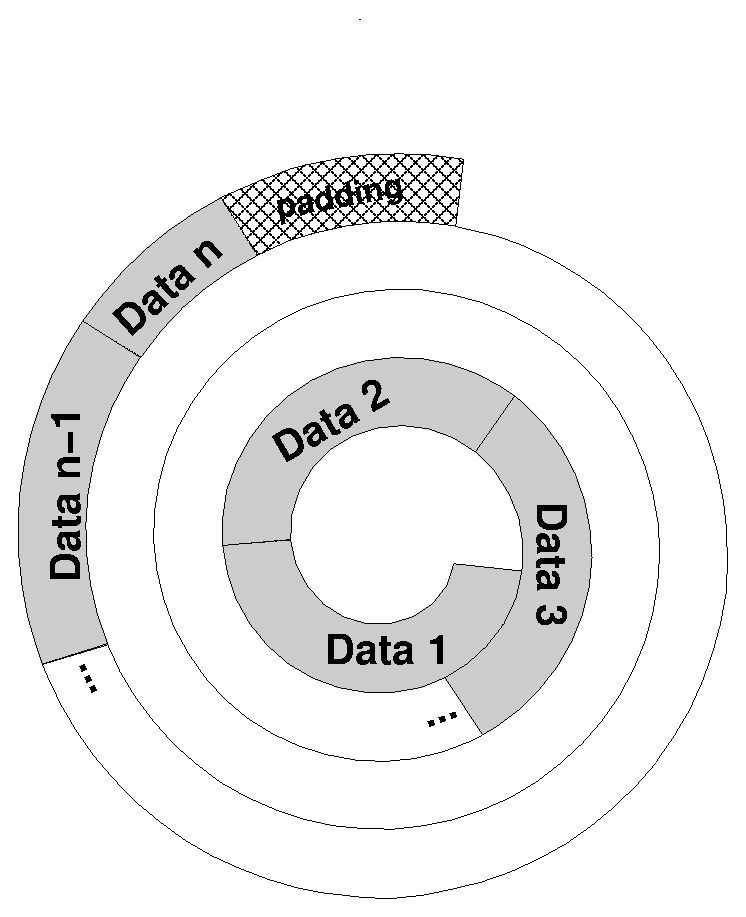
\includegraphics[width=67mm]{spiral-rs01.eps}
 \caption{Interpretation of physical layout in the .iso image}
 \label{layout-phy-one}
 \end{center}
\end{figure}

RS01 is meant to protect data which has already been written to an optical
medium, so the parity data can not be appended to the medium and must instead 
be kept in a separate error correction file. Like all dvdisaster
codecs, RS01 is based on a RS(255,k) Reed-Solomon code with  each
ecc block being comprised of $n$ data bytes and $k$ parity bytes, and
$n+k=255$.

The $n$ data bytes are taken from an iso image generated from the medium.
Reading data directly from the optical drive during encoding would slow down the
process tremendously due to massive random access over the medium, and 
quickly wear out the drive mechanics. However producing the .iso image 
takes one fast linear read, accesses the drive in a way it is designed to be used,
and puts the data on hard disk which can sustain the needed random access I/O.

Reed-Solomon codes
work best when errors are evenly distributed over all ecc blocks.
Therefore the $n$ data bytes used for creating an ecc block must be picked from
locations which are evenly distributed over the medium with a maximum
distance between each data byte pair. To obtain a suitable data distribution,
it is taken  into account that optical media are recorded as a single long 
spiral\footnote{Multiple layered
media contain one spiral for each physical layer, but are otherwise conceptually
identical.} of sectors each containing 2048 bytes.
The first sector lies at the innermost position of the spiral and is indexed with 0;
numbering continues onward to the outside of the spiral. The .iso image
contains a 1:1 mapping of this storage scheme, with the first 2048 bytes
holding the contents of sector 0, the next 2048 bytes resembling sector 1, and so on.

When encoding with $n$ data bytes per ecc block, the iso image is divided into
$n$ layers which physically map to the medium as shown in fig.\ref{layout-phy-one}. 
This distributes the ecc block reasonably good over the medium surface.
However since the image size does not need
to be a multiple of the layer size, the $n$-th layer may be physically shorter
as the layer size. For encoding purposes, the non-existant sectors in layer
$n$ are treated as sectors being filled with 2048 zero bytes. 

\subsection{Logical ecc file layout}

\begin{figure}
 \begin{center}
 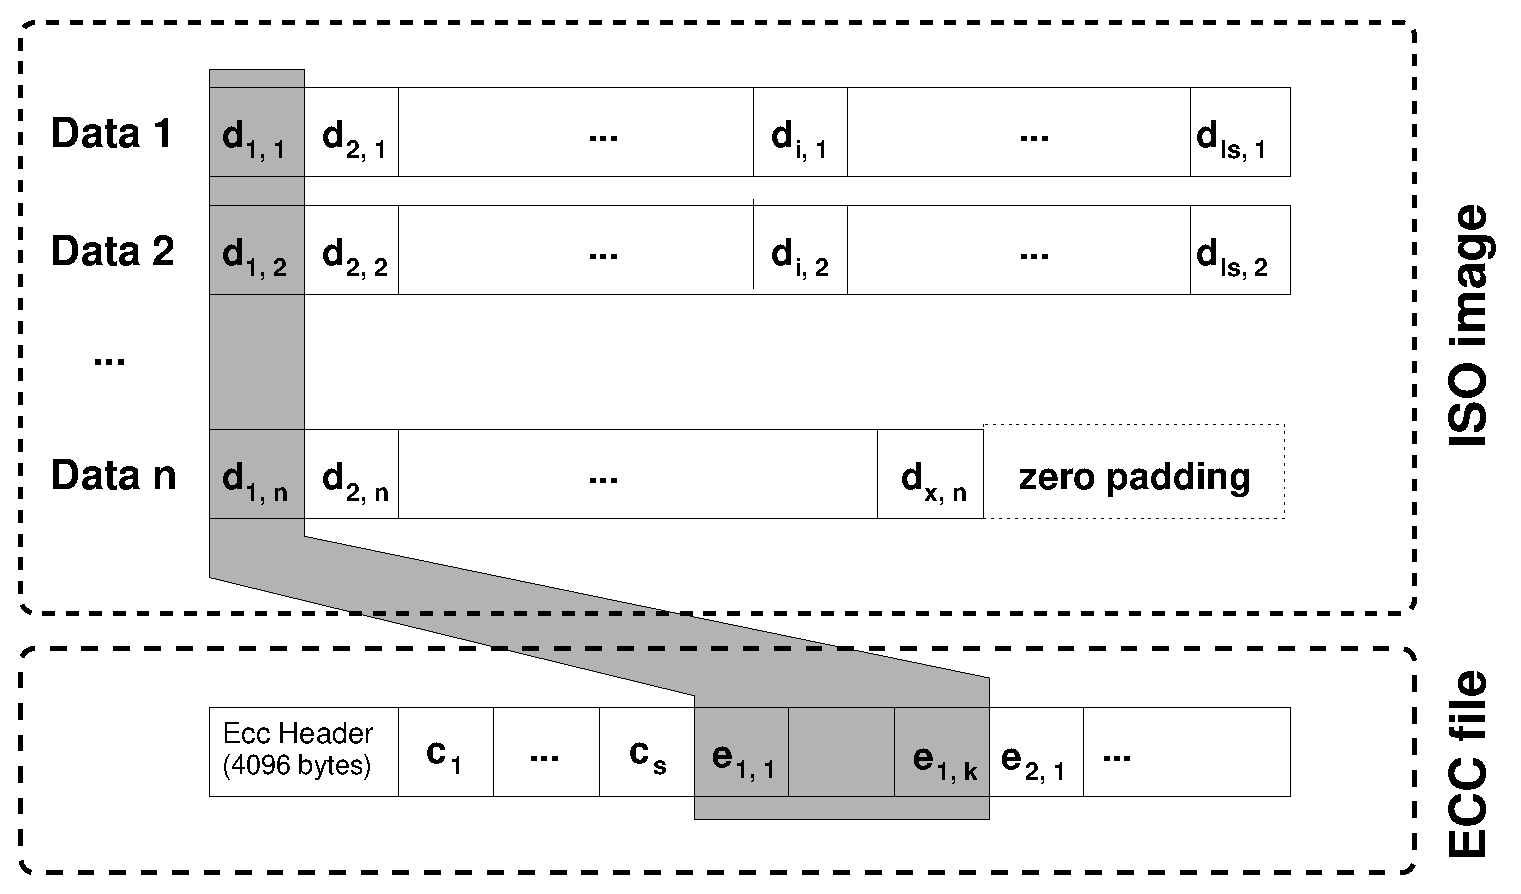
\includegraphics[width=\textwidth]{rs01-layout.eps}
 \caption{Logical RS01 layout}
 \label{layout-logical-one}
 \end{center}
\end{figure}

The ecc file layout, and therefore the relationship between the iso image
contents and the ecc file, is shown in 
figure \ref{layout-logical-one}. The first 4096 bytes of the ecc file
contain the ecc header whose format is described in appendix \ref{eh}.
For RS01, only the data fields marked with ``all'' or ``RS01'' are
relevant; all other fields should be set to zero.

Next to the ecc header comes the CRC section of the ecc file. If the
iso image contains $s$ sectors, the next $4*s$ bytes in the ecc file
contain the CRC32 sums of the sectors from the iso image: Let $b_1,\dots,b_{2048}$ denote 
the bytes of the first data sector; $b_{2049},\dots,b_{4096}$ those of the
second data sector and so on. Then $c_1 = CRC32(b_1,\dots,b_{2048})$,
$c_2 = CRC32(b_{2049},\dots,b_{4096})$ etc. Note that in contrast to
RS02 and RS03, bytes from the CRC section are not included into the ecc block
calculation and are therefore not protected by ecc.

\smallskip

The remainder of the ecc file contains the parity bytes of the
ecc blocks. For an ecc file built with $k$ roots, 
the iso image is logically divided into 
$n = 255-k$ layers as shown in figure \ref{layout-logical-one}.
The $d_{i,j}$ denote the $i-th$ byte in the $j-th$ layer.
In order to create the first ecc block, bytes $d_{1,1}$ to  $d_{1,n}$ are taken from the
$n$ layers. Then the RS(255,k) code is calculated (see appendix \ref{rs} for its parameters)
and the 
resulting $k$ parity bytes $e_{1,1}$ up to $e_{k,1}$ are stored
in the ecc file. The resulting ecc block is marked grey in the
figure. The next ecc blocks are calculated and stored accordingly.
In total, the ecc section contains $k*ls$ bytes of parity information,
with the $k$ parity bytes of each ecc block being stored consecutively.

\subsection{Calculating the layout for encoding}

The RS01 layout is fully determined by the number of roots for the error correction code
and the iso image size in sectors (from now on, ``size'' always means ``number of
2048K sectors). The number of roots can be freely chosen by the user from the
range of $[8...100]$. The iso image size is directly measured
from the iso image file.

\smallskip

The number of data layers is simply calculated from the number of roots, $k$:

\[ data\ layers = 255 - k\]

The size of each layer is:

\[ layer\ size = \left\lceil\frac{medium\ size}{data\ layers}\right\rceil\]

At the end of the last layer, $data\ layers * layer\ size - medium\ size$
zero filled padding sectors are used in the encoding process.

\subsection{Getting the layout when recovering defective media}

The required parameters are taken from the ecc header stored in
the error correction file (see appendix \ref{eh}). Especially,
the number of roots are taken from the {\em eccBytes} field and
the medium size is recorded in the {\em sectors} field.

\subsection{md5 checksums}

RS01 provides two md5 checksums for integrity checking.
The md5 sum of the iso image is calculated and stored in the
{\em mediumSum} field of the ecc header. 
Another md5 sum is calculated over the ecc file, excluding the
first 4096 bytes, and stored in the {\em eccSum} field of
the ecc header. It can be used to verify the integrity of the
ecc file itself. The ecc header is protected by its own CRC
checksum which is stored in the {\em selfCRC} field.

\smallskip

The md5 checksum generation is the major obstacle for parallelizing
the encoder. In RS03, md5sum generation has been made optional since
the RS03 layout allows suffcient consistency checks 
by doing a quick error syndrome check using the Reed-Solomon code.

\subsection{Special cases}

Error correction files can be created for any type of input files, not just iso files,
as long as the input files are ``reasonably'' long\footnote{Input files should contain
at least 2048*(255-k) bytes, so that there is at least one sector for each data
layer.}. Since input files are processed in units of 2048 kByte sectors, 
files whose byte size is not an integer multiple of 2048 are virtually padded 
with zeroes. In that case, the {\em inLast} field of the ecc header
contains the real byte size of the last file ``sector'' so that recovering the
last file sector does not write out the padding bytes. A size of zero in the
{\em inLast} field means that the last sector contains 2048 bytes.


% Header formats

\appendix

\appendix
\newpage
\section{The common Ecc header format}
\label{eh}

The ecc header is defined in the include file {\em dvdisaster.h}. 
Its C definition is as follows:

\begin{tabbing}
 xxx \= xxxxxxxxxxxxxxxxxxxxxxx \= xxx \kill
typedef struct \_EccHeader \\
\{\>gint8 cookie[12];           \>{\em /* "*dvdisaster*" */}\\
 \>gint8 method[4];            \>{\em /* e.g. "RS01" */}\\
 \>gint8 methodFlags[4];       \>{\em /* 0-2 for free use by the respective methods; 3 see above */}\\
 \>guint8 mediumFP[16];        \>{\em /* fingerprint of FINGERPRINT SECTOR */}\\ 
 \>guint8 mediumSum[16];       \>{\em /* complete md5sum of whole medium */}\\
 \>guint8 eccSum[16];          \>{\em /* md5sum of ecc code section of .ecc file */}\\
 \>guint8 sectors[8];          \>{\em /* number of sectors medium is supposed to have w/o ecc*/}\\
 \>gint32 dataBytes;           \>{\em /* data bytes per ecc block */}\\
 \>gint32 eccBytes;            \>{\em /* ecc bytes per ecc block */}\\
 \>gint32 creatorVersion;      \>{\em /* which dvdisaster version created this */}\\
 \>gint32 neededVersion;       \>{\em /* oldest version which can decode this file */}\\
 \>gint32 fpSector;            \>{\em /* sector used to calculate mediumFP */}\\
 \>guint32 selfCRC;            \>{\em /* CRC32 of EccHeader (currently RS02 only) -- since V0.66 --*/}\\
 \>guint8 crcSum[16];          \>{\em /* md5sum of crc code section of RS02 .iso file  */}\\
 \>gint32 inLast;              \>{\em /* bytes contained in last sector */}\\
 \>guint64 sectorsPerLayer;    \>{\em /* layer size for RS03 */}\\
 \>guint64 sectorsAddedByEcc;  \>{\em /* sectors added by RS02 */}\\
 \>gint8 padding[3960];        \>{\em /* pad to 4096 bytes: room for future expansion */}\\
\} EccHeader;
\end{tabbing}

\bigskip

The ecc header is used in all ecc formats (RS01, RS02, RS03) of dvdisaster,
but not all fields apply to all formats. See the following table for the meaning
and usage of the fields:
\bigskip

\begin{tabular}{|l|p{10cm}|c|}
\hline
Field & Usage & Format(s) \\
\hline
$cookie$ & Magic byte sequence for recognizing the header.\newline
Contains the string {\tt *dvdisaster*}. & all \\
\hline
$method$ & 4 characters describing the format; currently allowed:\newline
{\tt RS01}, {\tt RS02}, {\tt RS03}. & all \\ 
\hline
$methodFlags$ & 4 bytes for further specification of the format. &\\
 \cline{2-3} 
 & Byte 0 contains the following flag: &\\
 & Bit 0 - The {\em mediumSum} field is valid. & RS03 \\
 & Bit 1 - Set to 1 in ecc files. & RS03 \\
 \cline{2-3} 
 & Bytes 1-2 are unused in the current methods. & \\
 \cline{2-3} 
 & Byte 3 contains the following flags:\newline
Bit 0 - ecc data was created by a development release.\newline
Bit 1 - ecc data was created by a release candidate.\newline
If these bits are present, the user will be hinted that he is using
ecc data from a non-stable dvdisaster version. & all \\
\hline
\end{tabular}

{\footnotesize (continued on next page)}
\vfill
\newpage

\begin{tabular}{|l|p{10cm}|c|}
\hline
$mediumFP$ & The md5sum of the sector specified by the {\em fpSector}.
The sector should be chosen to have a huge probability being unique to the medium;
currently sector 16 (the ISO filesystem root sector) is used. & all \\
\hline
$mediumSum$ & The md5sum of the ISO image. For RS01 this is the md5sum of the
whole image; for RS02 it is calculated for the original ISO image (without
the added RS02 sectors). RS03 uses this value only when bit 1 in
{\em methodFlags} is set. & all \\ 
\hline
$eccSum$ & On RS01 this is the md5sum of the ecc file excluding the first 4096
bytes. For RS02 this is the md5sum calculated over the md5sums of the $nroots$
ecc layers. RS03 does not use this value. & RS01, RS02 \\
\hline
$sectors$ & For error correction files this is the number of sectors in the
protected medium. If augmented images are used, this denotes the number of
sectors in the original ISO image (without the added RS02/RS03 sectors). & all \\
\hline
$dataBytes$ & The number of data layers, including the CRC layer. & all \\
\hline
$eccBytes$ & The number of ecc layers (= number of roots) for the parity.
$dataBytes + eccBytes = 255$. & all\\
\hline
$creatorVersion$ & The dvdisaster version used for creating this ecc data.
A decimal value 102345 would mean dvdisaster version 10.23.45. & all \\
\hline
$neededVersion$ & The minimum dvdisaster version required for 
processing this ecc data. Version encoding as above. & all \\
\hline
$fpSector$ & The sector used for calculating $mediumFP$. & all \\
\hline
$selfCRC$ & A CRC32 checksum of the ecc header itself. Not used 
header fields are set to zero and the selfCRC field is initialized to the 
value 0x4c5047 (little endian). & \\
\hline
$crcSum$ & md5sum of the CRC layer in RS02 encoded images. & RS02 \\
\hline
$inLast$ & The number of Bytes contained in the last image sector. This allows for
encoding of files with arbitrary length, not just ISO images. 
dvdisaster versions prior to V0.66 do not use this field and always assume it
to be 2048 which is the default for iso images. & all \\
\hline
$sectorsPerLayer$ & The number of sectors per layer. & RS03 \\
\hline
$sectorsAddedByEcc$ & The total number of sectors (Headers, CRC, ECC) added. & RS02 \\
\hline
$padding$ & The ecc header is zero padded to a length of 4096 bytes. Future codes
may allocate additional space for the zero padding. See the note below for
usage of the upper 2048 bytes on RS02/RS03. & all \\
\hline
Byte 2048-4096 & A copy of the first CRC layer sector. & RS02 \\
\hline
\end{tabular}



\newpage
\section{RS03 CRC block format}
\label{crc-block}

The crc layer contains 2048 byte blocks containing the data structure
described below. Except for the CRC32 checksums most of the information
contained in this data structure is copied from the Ecc Header described
in appendix \ref{eh}. The crc block format is defined in the include 
file {\em dvdisaster.h} and has the following C definition:

\begin{tabbing}
 xxx \= xxxxxxxxxxxxxxxxxxxxxxx \= xxx \kill
typedef struct \_CrcBlock \\
\{\>guint32 crc[256];           \>{\em /* Checksum for the data sectors */}\\
\> gint8 cookie[12];            \>{\em /* "*dvdisaster*" */}\\
\> gint8 method[4];             \>{\em /* e.g. "RS03" */}\\
\> gint8 methodFlags[4];        \>{\em /* 0-2 for free use by the respective methods; 3 see above */}\\
\> gint32 creatorVersion;       \>{\em /* which dvdisaster version created this */}\\
\> gint32 neededVersion;        \>{\em /* oldest version which can decode this file */}\\
\> gint32 fpSector;             \>{\em /* sector used to calculate mediumFP */}\\
\> guint8 mediumFP[16];         \>{\em /* fingerprint of FINGERPRINT SECTOR */}\\ 
\> guint8 mediumSum[16];        \>{\em /* complete md5sum of whole medium */}\\
\> guint64 dataSectors;         \>{\em /* number of sectors of the payload (e.g. iso file sys) */}\\
\> gint32 inLast;               \>{\em /* bytes contained in last sector */}\\
\> gint32 dataBytes;            \>{\em /* data bytes per ecc block */}\\
\> gint32 eccBytes;             \>{\em /* ecc bytes per ecc block */}\\
\> guint64 sectorsPerLayer;     \>{\em /* for recalculation of layout */}\\
\> guint32 selfCRC;             \>{\em /* CRC32 of ourself, zero padded to 2048 bytes */}\\
\} CrcBlock;
\end{tabbing}

\bigskip

The CrcBlock data structure is used in the CRC layer of RS03 augmented images
only. RS02 has a similar CRC layer but uses a different concept for retrieving
layout information from the image. The following table describes the meaning
and usage of the CrcBlock fields:
\medskip

\begin{tabular}{|l|p{12cm}|}
\hline
Field & Usage \\
\hline 
crc & If this data structure is found in the {\em i-th} sector of the CRC layer,
it contains the CRC32 checksum for data sectors $d_{j,1}, \ldots, d_{j,n}$, with
$j = (i+1) \bmod\ layer\ size$. See figure \ref{layout-logical} for details.
Please note that the crc[] array is filled starting from crc[0], and unused field
are left zero. \\
\hline
$cookie$ & Magic byte sequence for recognizing the header.\newline
Contains the string {\tt *dvdisaster*}. \\
\hline
$method$ & 4 characters describing the format; currently only ``RS03''
may appear here.\\
\hline
\end{tabular}

{\footnotesize (continued on next page)}
\vfill
\newpage

\begin{tabular}{|l|p{12cm}|}
\hline
$methodFlags$ & 4 bytes for further specification of the format.\newline
Byte 0 contains the following flags:\newline
Bit 0 - The {\em mediumSum} field is valid.\newline
Bit 1 - Set to 1 in ecc files.\newline
Bytes 1-2 are unused in the current methods.\newline
Byte 3 contains the following flags:\newline
Bit 0 - ecc data was created by a development release.\newline
Bit 1 - ecc data was created by a release candidate.\newline
If these bits are present, the user will be hinted that he is using
ecc data from a non-stable dvdisaster version. \\
\hline
$creatorVersion$ & The dvdisaster version used for creating this ecc data.
A decimal value 102345 would mean dvdisaster version 10.23.45.\\
\hline
$neededVersion$ & The minimum dvdisaster version required for 
processing this ecc data. Version encoding as above. \\
\hline
$fpSector$ & The sector used for calculating $mediumFP$. \\
\hline
$mediumFP$ & The md5sum of the sector specified by the {\em fpSector}.
The sector should be chosen to have a huge probability being unique to the medium;
currently sector 16 (the ISO filesystem root sector) is used. \\
\hline
$mediumSum$ & The md5sum of the original ISO image if the first bit 
in the {\em methodFlags} field is set. Since md5sum generation can not be
parallelized, the user may opt not to calculate this checksum if multi core
encoding is used. \\
\hline
$dataSectors$ & For error correction files this is the number of sectors in the
protected medium. If augmented images are used, this denotes the number of
sectors in the original ISO image (without the added padding and RS03 sectors). \\
\hline
$inLast$ & The number of Bytes contained in the last image sector. This allows for
encoding of files with arbitrary length, not just ISO images.\\
\hline
$dataBytes$ & The number of data layers, including the CRC layer. \\
\hline
$eccBytes$ & The number of ecc layers (= number of roots) for the parity. \newline
$dataBytes + eccBytes = 255$. \\
\hline
$sectorsPerLayer$ & The number of sectors per layer. \\
\hline
$selfCRC$ & A CRC32 checksum of the ecc header itself. Not used fields are
set to zero and the selfCRC field is initialized to the 
value 0x4c5047 (little endian). \\
\hline
remaining bytes & The CrcBlock is zero padded to a size of 2048 bytes.\\
\hline
\end{tabular}


\newpage
\section{RS(255,k) encoding parameters and examples}
\label{rs}

dvdisaster uses a standard, non-shortened Reed-Solomon code
with the following commonly used parameters: \smallskip

The Galois field tables are generated by the field
generator polynomial 0x187 ($1 + X + X^2 + X^7 + X^8$).
The Reed-Solomon code generator polynomial is created using element 
0x70 as first consecutive root and the primitive element 0x0b. \medskip

As a starting point for testing your own implementation, some 
values and tables are shown below. The logarithm
and anti-logarithm tables in the Galois field are shown in tables
\ref{log-table} and \ref{anti-log-table}. Please note that there is no need for hard-coding
these tables as their contents can be enumerated by using
the field generator polynomial. \medskip

When encoding for 32 roots, the RS code generator polynomial will be:

{\small 01 5b 7f 56 10 1e 0d eb 61 a5 08 2a 36 56 ab 20 71 20 ab 56 36 2a 08 a5 61 eb 0d 1e 10 56 7f 5b 01}

or in index form:

{\small 00 f9 3b 42 04 2b 7e fb 61 1e 03 d5 32 42 aa 05 18 05 aa 42 32 d5 03 1e 61 fb 7e 2b 04 42 3b f9 00} \medskip

Using the above generator polynomial for encoding the data byte
sequence $\{0,1,\ldots,222\}$ produces the following parity bytes:

{\small 2f bd 4f b4 74 84 94 b9 ac d5 54 62 72 12 ee b3 eb ed 41 19 1d e1 d3 63 20 ea 49 29 0b 25 ab cf}

\newpage

\begin{table}
\begin{center}
\begin{tabular}{|l||c|c|c|c|c|c|c|c|c|c|c|c|c|c|c|c|}
\hline
&  00 & 01 & 02 & 03 & 04 & 05 & 06 & 07 & 08 & 09 & 0a & 0b & 0c & 0d & 0e & 0f \\
\hline
\hline
00 &  ff & 00 & 01 & 63 & 02 & c6 & 64 & 6a & 03 & cd & c7 & bc & 65 & 7e & 6b & 2a \\
\hline
10 &  04 & 8d & ce & 4e & c8 & d4 & bd & e1 & 66 & dd & 7f & 31 & 6c & 20 & 2b & f3 \\
\hline
20 &  05 & 57 & 8e & e8 & cf & ac & 4f & 83 & c9 & d9 & d5 & 41 & be & 94 & e2 & b4 \\
\hline
30 &  67 & 27 & de & f0 & 80 & b1 & 32 & 35 & 6d & 45 & 21 & 12 & 2c & 0d & f4 & 38 \\
\hline
40 &  06 & 9b & 58 & 1a & 8f & 79 & e9 & 70 & d0 & c2 & ad & a8 & 50 & 75 & 84 & 48 \\
\hline
50 &  ca & fc & da & 8a & d6 & 54 & 42 & 24 & bf & 98 & 95 & f9 & e3 & 5e & b5 & 15 \\
\hline
60 &  68 & 61 & 28 & ba & df & 4c & f1 & 2f & 81 & e6 & b2 & 3f & 33 & ee & 36 & 10 \\
\hline
70 &  6e & 18 & 46 & a6 & 22 & 88 & 13 & f7 & 2d & b8 & 0e & 3d & f5 & a4 & 39 & 3b \\
\hline
80 &  07 & 9e & 9c & 9d & 59 & 9f & 1b & 08 & 90 & 09 & 7a & 1c & ea & a0 & 71 & 5a \\
\hline
90 &  d1 & 1d & c3 & 7b & ae & 0a & a9 & 91 & 51 & 5b & 76 & 72 & 85 & a1 & 49 & eb \\
\hline
a0 &  cb & 7c & fd & c4 & db & 1e & 8b & d2 & d7 & 92 & 55 & aa & 43 & 0b & 25 & af \\
\hline
b0 &  c0 & 73 & 99 & 77 & 96 & 5c & fa & 52 & e4 & ec & 5f & 4a & b6 & a2 & 16 & 86 \\
\hline
c0 &  69 & c5 & 62 & fe & 29 & 7d & bb & cc & e0 & d3 & 4d & 8c & f2 & 1f & 30 & dc \\
\hline
d0 &  82 & ab & e7 & 56 & b3 & 93 & 40 & d8 & 34 & b0 & ef & 26 & 37 & 0c & 11 & 44 \\
\hline
e0 &  6f & 78 & 19 & 9a & 47 & 74 & a7 & c1 & 23 & 53 & 89 & fb & 14 & 5d & f8 & 97 \\
\hline
f0 &  2e & 4b & b9 & 60 & 0f & ed & 3e & e5 & f6 & 87 & a5 & 17 & 3a & a3 & 3c & b7 \\
\hline
\end{tabular}
\end{center}
\caption{Galois field logarithm table}
\label{log-table}
\end{table}

\bigskip

\begin{table}
\begin{center}
\begin{tabular}{|l||c|c|c|c|c|c|c|c|c|c|c|c|c|c|c|c|}
\hline
&  00 & 01 & 02 & 03 & 04 & 05 & 06 & 07 & 08 & 09 & 0a & 0b & 0c & 0d & 0e & 0f \\
\hline
\hline
00 &  01 & 02 & 04 & 08 & 10 & 20 & 40 & 80 & 87 & 89 & 95 & ad & dd & 3d & 7a & f4 \\
\hline
10 &  6f & de & 3b & 76 & ec & 5f & be & fb & 71 & e2 & 43 & 86 & 8b & 91 & a5 & cd \\
\hline
20 &  1d & 3a & 74 & e8 & 57 & ae & db & 31 & 62 & c4 & 0f & 1e & 3c & 78 & f0 & 67 \\
\hline
30 &  ce & 1b & 36 & 6c & d8 & 37 & 6e & dc & 3f & 7e & fc & 7f & fe & 7b & f6 & 6b \\
\hline
40 &  d6 & 2b & 56 & ac & df & 39 & 72 & e4 & 4f & 9e & bb & f1 & 65 & ca & 13 & 26 \\
\hline
50 &  4c & 98 & b7 & e9 & 55 & aa & d3 & 21 & 42 & 84 & 8f & 99 & b5 & ed & 5d & ba \\
\hline
60 &  f3 & 61 & c2 & 03 & 06 & 0c & 18 & 30 & 60 & c0 & 07 & 0e & 1c & 38 & 70 & e0 \\
\hline
70 &  47 & 8e & 9b & b1 & e5 & 4d & 9a & b3 & e1 & 45 & 8a & 93 & a1 & c5 & 0d & 1a \\
\hline
80 &  34 & 68 & d0 & 27 & 4e & 9c & bf & f9 & 75 & ea & 53 & a6 & cb & 11 & 22 & 44 \\
\hline
90 &  88 & 97 & a9 & d5 & 2d & 5a & b4 & ef & 59 & b2 & e3 & 41 & 82 & 83 & 81 & 85 \\
\hline
a0 &  8d & 9d & bd & fd & 7d & fa & 73 & e6 & 4b & 96 & ab & d1 & 25 & 4a & 94 & af \\
\hline
b0 &  d9 & 35 & 6a & d4 & 2f & 5e & bc & ff & 79 & f2 & 63 & c6 & 0b & 16 & 2c & 58 \\
\hline
c0 &  b0 & e7 & 49 & 92 & a3 & c1 & 05 & 0a & 14 & 28 & 50 & a0 & c7 & 09 & 12 & 24 \\
\hline
d0 &  48 & 90 & a7 & c9 & 15 & 2a & 54 & a8 & d7 & 29 & 52 & a4 & cf & 19 & 32 & 64 \\
\hline
e0 &  c8 & 17 & 2e & 5c & b8 & f7 & 69 & d2 & 23 & 46 & 8c & 9f & b9 & f5 & 6d & da \\
\hline
f0 &  33 & 66 & cc & 1f & 3e & 7c & f8 & 77 & ee & 5b & b6 & eb & 51 & a2 & c3 & 00 \\
\hline
\end{tabular}
\end{center}
\caption{Galois field anti-logarithm table}
\label{anti-log-table}
\label{LastPage}
\end{table}

\end{document}
